\documentclass[10pt]{article}
\usepackage[margin=0.9in]{geometry}
\usepackage{amsmath, amssymb, amsfonts}
\usepackage{graphicx}
\usepackage{booktabs}
\usepackage{longtable}
\usepackage{array}
\usepackage{float}
\usepackage{caption}
\usepackage{xcolor}
\usepackage{enumitem}
\usepackage[T1]{fontenc}
\usepackage{lmodern}
\usepackage{textcomp}
\usepackage{url}
\newcommand{\pathtt}[1]{\texttt{\path{#1}}}
\usepackage[hidelinks]{hyperref}
\captionsetup{font=small, labelfont=bf, width=0.96\textwidth}
\setlength{\parskip}{4pt}
\sloppy
\setlength{\emergencystretch}{3em}
\newcommand{\pstar}{p^\star}
\newcommand{\perr}{\lVert p - \pstar\rVert}
\newcommand{\readthis}[1]{\textbf{Read this:} #1}
\newcommand{\fig}[1]{\texttt{figures/#1}}

\title{R002 --- Figure atlas: multiple shooting with guess propagation for sparse model selection\\
\large Concept figures, fresh simulations supporting the theory, solver/optimiser/parameter variations,\\ and the repository defects that were found and fixed}
\author{Prepared for Manu Jayadharan\\ \small report folder \path{reports/2026-09-11-R002-multishooting-figure-atlas/}}
\date{11 September 2026\\ \small Part~I (extended landscape animations) added 12 September 2026}

\begin{document}
\maketitle

\begin{abstract}
\noindent This atlas collects, in presentation order, every figure produced for the \texttt{hiddenSelect} project (Julia; multiple shooting with guess propagation for discovering sparse polynomial governing equations from noisy trajectories; theory manuscript \emph{Sparse Optimization using Multi-Shooting and Guess Propagation}). It contains: (i) seven concept figures that replace the manuscript's hand-drawn sketches (the inverse problem, single shooting, the shooting partition, multiple shooting, node removal, the guess-propagation algorithm, and the error-growth picture); (ii) numerical checks of Lemma~1, Lemma~2 and Proposition~1 of the manuscript on the FitzHugh--Nagumo (FHN) system; (iii) cost-landscape figures showing how the number of local minima, the Hessian spread and the blow-up region grow with the window size; (iv) the headline experiment --- guess propagation versus restarting from the seed --- over 8 optimiser seeds with paired bootstrap confidence intervals, plus variations of the window-size schedule, blow-up penalty, noise level, sparsity weight, optimiser, iteration budget, integrator sub-steps and start distance; (v) an integrator/solver comparison; (vi) the quantification of the defects reported in the code review R001 (F1, F2, F4, F5) and of two \emph{new} defects found here (a mixed monomial ordering in the current driver and a global-variable shadowing in the single-shooting loss), all fixed in the live tree with this report; (vii) the same method on Lotka--Volterra and Lorenz. Every number in every caption is computed by scripts in this folder from a frozen code snapshot and asserted by 20 gates (\S\ref{sec:gates}); twenty MP4 animations (including a screened set of five FHN cost-landscape planes at $201\times201$ and four rotating 3-D landscapes, \S\ref{sec:anim2}) and a slide deck are shipped alongside. Headline: with guess propagation the median parameter error over seeds falls from $1.65$ (seed) to $0.32$ at full single shooting, while the same optimiser without propagation stays at the seed ($1.65$) --- paired difference $-1.14$, 95\,\% bootstrap CI $[-1.43,-0.77]$, better in 7 of 8 seeds (the eighth seed starts on the blow-up plateau, where nothing can move; a graded penalty fixes that).
\end{abstract}

\section*{Table of figures}
\addcontentsline{toc}{section}{Table of figures}
\small
\begin{longtable}{p{0.06\textwidth} p{0.39\textwidth} p{0.46\textwidth}}
\toprule
Figure & What is plotted & What it demonstrates / how to use it on a slide \\
\midrule
\endhead
\multicolumn{3}{l}{\emph{A. Concept figures (replace the hand-drawn sketches of the manuscript)}}\\
\ref{fig:01} & FHN trajectory, noisy samples, phase portrait, the $2\times10$ sparse coefficient matrix & The inverse problem: recover the few non-zero library coefficients from noisy samples. Opening slide.\\
\ref{fig:02} & Single-shooting model trajectory from $y_0$ at a wrong $p$, residual lines, $|{\rm residual}|$ vs $t$ & Why single shooting is hard: the initial-condition error is amplified like $e^{Lt}$ over the whole record.\\
\ref{fig:03} & Timeline of data times $t_i$, shooting nodes $\tau_k$, windows, $\Delta t$, $\Delta T$; the coarser partition below & The shooting partition and what ``removing a node'' means (replaces \texttt{shooting\_partition.png}).\\
\ref{fig:04} & Single vs multiple shooting ($\kappa=100,10,5$) at the same wrong $p$, per-window segments, residuals & Restarting at the nodes caps the error at $e^{L\Delta T}$ (replaces \texttt{multiple\_shooting.png}).\\
\ref{fig:05} & Fine vs coarse partition around a removed node, $\Delta T_1$, $\Delta T_2$, the bound of Prop.~1 & Node removal: what changes in the cost when one node is dropped (replaces \texttt{comparison\_shooting\_nodes.png}).\\
\ref{fig:06} & 1-D cost slices for $\kappa=1,5,25,100$ with the minimiser carried forward; pseudo-code & The guess-propagation algorithm: solve the smooth problem first, carry its minimiser into the rugged ones.\\
\ref{fig:07} & Schematic error envelopes $e^{Lt}\lVert\eta\rVert$ vs the sawtooth capped at $e^{L\Delta T}\lVert\eta\rVert$ & The one-line argument for multiple shooting (uses the report's $L$ and $\lVert\eta\rVert_{\max}$).\\
\midrule
\multicolumn{3}{l}{\emph{B. Numerical checks of the theory}}\\
\ref{fig:08} & $\lVert\varphi(t;x_1)-\varphi(t;x_2)\rVert/\lVert x_1-x_2\rVert$ for 24 probes vs $e^{\pm Lt}$, $e^{\mu t}$ & Lemma~1 holds; the Lipschitz bound is very loose on the FHN limit cycle (actual amplification $\le 8$).\\
\ref{fig:09} & $\lVert\varphi(t;p_1)-\varphi(t;p_2)\rVert/\lVert p_1-p_2\rVert$ vs the Lemma~2 bound & Lemma~2 holds; parameter sensitivity saturates instead of growing exponentially.\\
\ref{fig:10} & $|\hat J_K-J_K|$ vs number of removed nodes and vs $\Delta T_2$ & Proposition~1 qualitatively: the cost change grows with $|I_R|$ and with $\Delta T_2$; remove few nodes at a time.\\
\midrule
\multicolumn{3}{l}{\emph{C. Cost landscapes}}\\
\ref{fig:11} & 2-D slices of $J_\kappa$ in the ($v$, $v^3$) coefficient plane of $\dot v$, $\kappa=1,3,10,100$ & The basin narrows and a blow-up plateau appears as $\kappa$ grows; a positive cubic coefficient blows up in finite time.\\
\ref{fig:12} & Same in the ($w$ in $\dot v$, $v$ in $\dot w$) plane & The slow $\dot w$ equation is weakly identifiable at small $\kappa$ and better at large $\kappa$.\\
\ref{fig:13} & 1-D slices along random directions; local-minima count vs $\kappa$ & Local minima per slice grow from 1.3 ($\kappa=1$) to 7.9 ($\kappa=100$).\\
\ref{fig:14} & Hessian $\lambda_{\max}$, $|\lambda_{\min}|$, $\lVert\nabla J_\kappa(\pstar)\rVert$, number of negative eigenvalues vs $\kappa$; sensitivity to $x_0$ & Conditioning worsens by $10^{4.5}$ and the noisy cost becomes indefinite at $\pstar$ for $\kappa\ge2$.\\
\midrule
\multicolumn{3}{l}{\emph{D. Guess propagation: the headline experiment (8 seeds)}}\\
\ref{fig:15} & $J_\kappa$, $\perr$ and recovery score vs $\kappa$ for GP, best-guess GP and no propagation & The claim of the paper, with seeds shown: GP reaches single shooting with $\perr\approx0.32$; the control never leaves the seed.\\
\ref{fig:16} & Paired differences GP $-$ control with bootstrap CIs; cellwise counts & The difference is decisive at every $\kappa\ge2$ (7 of 8 seeds; CI excludes 0).\\
\ref{fig:17} & Seed-median coefficient error heat-map along the sweep & Which coefficients are recovered when; the $w$ coefficient of $\dot v$ is shrunk by the sparsity term.\\
\ref{fig:18} & Filmstrip of single-shooting fits from the minimiser at $\kappa=1,5,25,100$, GP vs control (seed 2) & Visual companion of \ref{fig:15}; still frames of \texttt{anim\_sweep.gif}.\\
\ref{fig:19} & Nelder--Mead cost traces per $\kappa$ (seed 2), GP vs control & GP starts every stage near its optimum; the control stalls on the plateau.\\
\ref{fig:20} & Final coefficients at $\kappa=100$ vs truth, all seeds & Correctly labelled coefficient bar chart (the repository's labels were stale).\\
\midrule
\multicolumn{3}{l}{\emph{E. Variations}}\\
\ref{fig:21} & Window-size schedule: dense (44 steps), full (16), coarse (4), jump (2) & Removing few nodes per step matters: jump $0.76$ vs dense $0.30$ median error.\\
\ref{fig:22} & Flat vs graded blow-up penalty & The graded penalty removes the ``stuck on the plateau'' failure (0 vs 12.5\,\% of seeds).\\
\ref{fig:23} & Noise level $\sigma_{\rm rel}\in\{0,\dots,0.2\}$ & GP is robust up to 10\,\% noise and fails at 20\,\%; the control fails even at zero noise.\\
\ref{fig:24} & Sparsity weight $\gamma$ & $\gamma=0.05$ is best; $\gamma=0$ and $\gamma=1$ both hurt; which coefficients survive.\\
\ref{fig:25} & Nelder--Mead vs BFGS vs L-BFGS (AD gradient through the windowed loss) & With the F4 fix, BFGS+GP is the best and cheapest arm ($\perr=0.21$, score $0.95$); gradients die on the plateau.\\
\ref{fig:26} & Basin of attraction of one window size vs start distance & Small windows have wide basins but a noise-limited floor; single shooting has a narrow basin.\\
\ref{fig:27} & Nelder--Mead iteration budget; integrator sub-steps $S$ & 2500 iterations are needed; $S\ge5$ suffices; $S=1$ biases the fit.\\
\ref{fig:28} & Start scale $0.01$--$0.3$, flat vs graded penalty & Farther starts are harder; the graded penalty rescues starts that begin on the plateau.\\
\midrule
\multicolumn{3}{l}{\emph{F. Integrators and solvers inside the loss}}\\
\ref{fig:29} & Accuracy vs cost per loss evaluation for 14 integrator settings & The in-house fixed-step Tsit5 ($S=10$) matches a $10^{-12}$ reference to $10^{-13}$ and is the cheapest accurate choice; the problem is not stiff.\\
\ref{fig:30} & GP sweep with three integrators inside the loss & The integrator does not change the outcome; the plateau start (seed 1) does.\\
\midrule
\multicolumn{3}{l}{\emph{G. Defects found and fixed}}\\
\ref{fig:31} & F2: share of the loss dropped by the mod~7 stiff branch; 1-D slice through the $\dot w$ equation & 9--17\,\% of $J(\pstar)$ and up to 78\,\% away from $\pstar$ was silently discarded; fixed.\\
\ref{fig:32} & F1: Jacobian entry, eigenvalues and trace from the truncated vs fixed RHS & The stability movies used $\partial\dot v/\partial v=+1.0$ instead of $-1.25$; fixed.\\
\ref{fig:33} & F4: cosine between the gradient the sweep received and the right one; BFGS with each & Near-orthogonal at $\kappa=1$; BFGS stalls with the wrong gradient; fixed.\\
\ref{fig:34} & New: mixed monomial order in the mod~8 driver; global-data shadowing & A spurious $\perr=2.50$ and an ignored argument; both fixed.\\
\midrule
\multicolumn{3}{l}{\emph{H. Other systems and closing the loop}}\\
\ref{fig:35} & Lotka--Volterra (12 coefficients) & GP recovers the system ($\perr=0.29$, score 0.83); the control blows up in 5 of 6 seeds.\\
\ref{fig:36} & Lorenz (30 coefficients, chaotic) & GP+BFGS recovers Lorenz (score 0.83); GP+Nelder--Mead does not converge; the control fails in 4 of 4 seeds.\\
\ref{fig:37} & Hessian at the GP minimisers; cost along the segment between consecutive minimisers; cross-evaluation & The strong-convexity premise is not verified at Nelder--Mead's returned iterates (positive definite in 36\,\% of cells); the carried guess sits inside the next basin.\\
\bottomrule
\end{longtable}
\normalsize
\noindent Animations (MP4, H.264; frames regenerable by \texttt{figures/make\_animations.py} and, for the last two groups, \texttt{figures/make\_landscape\_animations.py}; the GIF \texttt{anim\_sweep.gif} is the same content as the first one). The first nine are $825\times616$; the extended landscape set of \S\ref{sec:anim2} is $2560\times1440$:
\begin{itemize}[leftmargin=1.4em, itemsep=0pt]
\item \texttt{figures/anim\_fhn\_sweep.mp4} --- FHN: $v(t)$ fit from the minimiser at every stage, GP vs control (seed 2), with the running cost and error.
\item \texttt{figures/anim\_fhn\_phase.mp4} --- FHN: the same sweep in the $(v,w)$ phase plane with the coefficient bars against the truth.
\item \texttt{figures/anim\_fhn\_multiple\_shooting.mp4} --- concept: single shooting drawn forward in time at a wrong $p$, then the $\kappa=10$ windows appearing one by one, then node removal ($\kappa=1\to100$) with the cost of the wrong and true $p$.
\item \texttt{figures/anim\_fhn\_landscape.mp4} --- FHN: the 2-D cost landscape in the $(v,v^3)$ plane morphing through every stage of the FULL schedule, with the GP and control paths (seed 2) overlaid (data: \texttt{anim\_landscape\_v\_v3.csv}, script \texttt{analysis/10\_animation\_data.jl}).
\item \texttt{figures/anim\_lv\_sweep.mp4}, \texttt{figures/anim\_lv\_phase.mp4} --- Lotka--Volterra: $x(t),y(t)$ fits, phase plane and coefficients along the sweep, GP vs control (seed 1).
\item \texttt{figures/anim\_lv\_landscape.mp4} --- Lotka--Volterra: the 2-D cost landscape in the ($x$, $xy$) coefficient plane of $\dot x$ morphing through every FULL window size, with the GP and control paths (seed 1) overlaid (data: \texttt{anim\_lv\_landscape\_x\_xy.csv}, script \texttt{analysis/11\_lv\_landscape.jl}).
\item \texttt{figures/anim\_lv\_landscape\_x2\_xy.mp4}, \texttt{figures/anim\_lv\_landscape\_xy\_xy.mp4} --- the same at $161\times161$ resolution in two more planes: ($x^2$, $xy$) of $\dot x$, where the true-zero quadratic term produces finite-time blow-up (the analogue of the FHN cubic: a smooth diagonal valley at $\kappa=1$ shatters into a thin sliver with secondary minima at $\kappa=100$), and the interaction pair ($xy$ in $\dot x$, $xy$ in $\dot y$), where a round bowl becomes an L-shaped plateau (data: \texttt{anim\_lv\_landscape\_x2\_xy.csv}, \texttt{anim\_lv\_landscape\_xy\_xy.csv}).
\item \textbf{Extended 2-D landscapes} (\S\ref{sec:anim2}; $201\times201$ grids, 1440p; data \texttt{anim\_fhn\_landscape\_*.csv.gz}, \texttt{anim\_lv\_landscape\_x2\_xy\_hires.csv.gz}, script \texttt{analysis/12\_landscape\_planes.jl}) --- \texttt{anim\_fhn\_landscape\_v\_v3\_hires.mp4} (the Part~C plane at the new resolution), \texttt{..\_wv\_ww\_hires.mp4} ($v$ and $w$ in $\dot w$: the slow block, nearly flat at $\kappa=1$), \texttt{..\_v2\_w2\_hires.mp4} ($v^2$ in $\dot v$ and in $\dot w$: two true zeros, plateau $0\to57\,\%$), \texttt{..\_w\_wv\_hires.mp4} ($w$ in $\dot v$, $v$ in $\dot w$: the feedback pair; sharpens hard but barely blows up --- plateau $0\,\%$ for every $\kappa\le33$, $0.27\,\%$ at $\kappa=100$), \texttt{..\_v3\_w3\_hires.mp4} ($v^3$ in $\dot v$ and in $\dot w$: rugged at both ends), and \texttt{anim\_lv\_landscape\_x2\_xy\_hires.mp4}. Each frame also carries the basin and plateau fractions of that $\kappa$.
\item \textbf{3-D landscapes} (\S\ref{sec:anim2}; rotating surface $z=\log_{10}J_\kappa$, one full turn over 288 frames) --- \texttt{anim3d\_fhn\_landscape\_wv\_ww.mp4}, \texttt{anim3d\_fhn\_landscape\_v2\_w2.mp4}, \texttt{anim3d\_fhn\_landscape\_v\_v3.mp4} and \texttt{anim3d\_lv\_landscape\_x2\_xy.mp4}. The surface is clipped at the 99.5th percentile of the finite costs for display; see the display convention in \S\ref{sec:anim2}.
\item \textbf{3-D landscape without guess propagation} --- \texttt{anim3d\_fhn\_landscape\_wv\_ww\_control.mp4}: the same slow-block surface as \texttt{anim3d\_fhn\_landscape\_wv\_ww.mp4} with the guess-propagation path removed, showing only the minimiser the optimiser returns at each $\kappa$ when every stage restarts from the same seed --- what the method does \emph{before} guess propagation is introduced. The gutter panel carries that arm's $\lVert p^{(\kappa)}-p^\star\rVert$ along the ladder.
\end{itemize}
A slide deck telling the story in 8 slides is in \texttt{slides/multishooting\_story.pptx} (built by \texttt{slides/make\_deck.py} from these figures and \texttt{tables/table\_numbers.json}). Every figure exists as PDF and PNG under \texttt{figures/}.

\tableofcontents

\section{Introduction}
The code-review report R001 (10 September 2026) established that the repository's central claim reproduces and listed seven defects. This report is the figure companion for a presentation. It adds three things R001 did not have: proper concept figures for the method (Part~A), a broad batch of \emph{fresh} simulations run in parallel (522 optimisation sweeps over 8 seeds and 9 variation axes, plus two other dynamical systems) that support or qualify the theory's claims (Parts B--F, H), and the quantification \emph{and fix} of the defects, with before/after figures (Part~G). Nothing is re-used from R001: every quantity that overlaps (the headline sweep, the F1/F2 numbers) is recomputed here from a frozen snapshot of the sources, and the bug figures execute the pre-fix and post-fix code side by side.

Two things the reader should keep in mind. First, the optimiser seed matters enormously and is reported everywhere: one of the eight random starts lands on the blow-up plateau at the very first window size and never moves under the repository's flat penalty (\S\ref{sec:gp}); it is kept in every statistic rather than dropped. Second, the sweep in the committed driver (\texttt{fhn\_model\_selection\_mod 8.jl}) had guess propagation \emph{disabled} and used two different monomial orderings for the sweep and the polish (\S\ref{sec:bugs}); the driver is fixed in the same commit as this report.

\section{Definitions (read before the figures)}\label{sec:defs}
Everything used in a caption is defined here, including terms inherited from the manuscript and from R001.

\subsection{Model, library and data}
The target is FitzHugh--Nagumo,
\begin{equation}
\dot v = v - \tfrac{1}{3}v^3 - w + 0.5,\qquad \dot w = \tfrac{1}{12.5}\,(v + 0.7 - 0.8\,w),
\end{equation}
written as a general two-dimensional cubic polynomial system so that model \emph{selection} (which monomials are present) is part of the task:
\begin{equation}
\dot x_i = \sum_{j=1}^{J} p_{ij}\,\Theta_j(\mathbf x),\quad i=1,2,\qquad
\Theta = \{1,\ w,\ w^2,\ w^3,\ v,\ vw,\ vw^2,\ v^2,\ v^2 w,\ v^3\},\quad J=10 .
\end{equation}
\readthis{the library order above is the \emph{multi-index} order produced by \texttt{helper\_functions.jl} and used by \texttt{odefun\_poly!} (mod~8). The older hard-coded RHS \texttt{odefun} (mods~2--7) uses the order $1,v,w,v^2,vw,w^2,v^3,v^2w,vw^2,w^3$. The two orders are different permutations of the same 10 monomials; mixing them is finding N1 in \S\ref{sec:bugs}. All coefficient plots here use the library order, with the $\dot v$ block (10 entries) followed by the $\dot w$ block.} The parameter vector $p\in\mathbb R^{20}$ has 6 non-zero entries: $\dot v$: $(1)\!=\!0.5$, $(w)\!=\!-1$, $(v)\!=\!1$, $(v^3)\!=\!-1/3$; $\dot w$: $(1)\!=\!0.056$, $(w)\!=\!-0.064$, $(v)\!=\!0.08$ (seven including the $\dot w$ constant). The optimisation vector is $z=[x_0;\,p]\in\mathbb R^{22}$: the first two entries are a free initial condition that enters only through the term $\lVert x_0-y_0\rVert^2$.

Data follow the repository recipe exactly (frozen mod~8 lines 103--157, reproduced to $6\times10^{-15}$, gate G3): integrate with the in-house fixed-step Tsit5 at $\delta t_{\rm fine}=0.01$ from $(1,1)$ to $T=156$, keep every 100th point, crop to $t\in[50,150]$ and shift to $t\in[0,100]$ ($N=101$ samples, spacing $\Delta t=1$), and add Gaussian noise to each component with standard deviation $0.05\times$ that component's own standard deviation (seed 1287436679). The resulting maximum noise norm is $\lVert\eta\rVert_{\max}=0.159$ and the noise floor of the data term is $\tfrac1N\sum_i\lVert\eta_i\rVert^2=0.0052$.

\subsection{Cost function}
For a window size $\kappa$ (number of data intervals per window, $1\le\kappa\le N-1$) the record is cut into $K=\lceil (N-1)/\kappa\rceil$ windows; each window is integrated \emph{from the noisy datum at its left node} with $S$ fixed Tsit5 sub-steps of length $\delta t=\Delta t/S$ per data interval, and
\begin{equation}
J_\kappa(z)=\frac{1}{N}\Big[\lVert x_0-y_0\rVert^2+\sum_{i=1}^{N-1}\big\lVert \hat x(t_{i+1};\,p,\,y_{\tau(i)})-y_{i+1}\big\rVert^2\Big]+\frac{\gamma}{20}\sum_{j=1}^{20}\operatorname{smooth}\ell_1(p_j),
\label{eq:J}
\end{equation}
where $\tau(i)$ is the last node at or before $t_i$, and $\operatorname{smooth}\ell_1(x)=\alpha^{-1}[\log(1+e^{-\alpha x})+\log(1+e^{\alpha x})]$ with $\alpha=500$ (equal to $|x|$ for $|\alpha x|>40$). $\kappa=1$ is one window per data interval; $\kappa=N-1=100$ is single shooting. \readthis{node states are \emph{not} optimisation variables and no continuity constraint is imposed (unlike textbook multiple shooting); this is the manuscript's formulation and the repository's code.} If any state exceeds $10^3$ in magnitude or becomes NaN during integration, the loss returns the constant $10^3$ (\emph{flat blow-up penalty}, a plateau with zero gradient). The \emph{graded} penalty (a variant introduced here) returns $10^3\,(1+\tfrac{N-1-i}{N-1})+J_{\rm partial}/N$ when the blow-up occurs at data index $i$, so that later blow-ups cost less and a derivative-free optimiser has a direction. The manuscript's $J_K$ (no normalisation, no sparsity term) differs from (\ref{eq:J}) by the factor $1/N$ and the $\gamma$ term; the theory figures (Part~B) use $\gamma=0$.

\subsection{Arms}
\begin{description}[leftmargin=1.6em, itemsep=1pt]
\item[GP (guess propagation)] Sweep $\kappa$ upward through a schedule; the minimiser of each stage is the start of the next. Schedules: FULL $=\{1,2,3,4,5,6,8,10,12,15,20,25,33,50,75,\allowbreak 100\}$ (default); SHORT $=\{1,2,5,10,25,50,100\}$ for the variation experiments; DENSE $=\{1,\dots,30,35,40,\dots,100\}$ (44 stages); COARSE $=\{1,5,25,100\}$; JUMP $=\{1,100\}$.
\item[best-GP] As GP but the start of the next stage is the best (lowest-cost) minimiser seen so far.
\item[control (no propagation)] Every stage starts from the same random seed vector. This is the arm the committed mod~8 driver was running.
\item[optimiser] Nelder--Mead (Optim.jl, 2500 iterations, default tolerances) unless stated; BFGS and L-BFGS use the exact ForwardDiff gradient of (\ref{eq:J}) through the integrator (possible only after fix F4), same iteration cap, $g_{\rm tol}=10^{-8}$.
\item[seed] Optimiser seed $s\in\{1,\dots,8\}$: $z_{\rm seed}=[y_0;\ 0.1\,\xi]$, $\xi\sim\mathcal N(0,I_{20})$ from \texttt{MersenneTwister}$(s)$; $\lVert p_0-\pstar\rVert\in[1.50,1.84]$ over the 8 seeds (0.1 is R001's scale; the repository uses 0.01 --- see \ref{fig:28}).
\end{description}
\readthis{arms are compared at \emph{equal} budgets (same iterations, same schedule, same seeds) except where the figure says otherwise: the schedule experiment (\ref{fig:21}) deliberately changes the number of stages, and the optimiser experiment (\ref{fig:25}) reports wall time because the gradient methods do different work per iteration.}

\subsection{Metrics}
\begin{description}[leftmargin=1.6em, itemsep=1pt]
\item[$J_\kappa$ (primary)] the cost (\ref{eq:J}) at the returned minimiser, including the sparsity term; $J_\kappa\ge10^3$ flags a blow-up (\emph{plateau}). Costs at different $\kappa$ are not directly comparable (different restarts).
\item[$\perr$] Euclidean distance between the fitted 20-vector and the true coefficients; the identification metric. Not computed by the repository; the same definition as R001.
\item[recovery score] fractional system-recovery score in $[0,1]$: each of the 20 coefficients earns credit 1 if it is correctly zero ($|p_j|<0.05$ when $\pstar_j=0$) or correctly non-zero within 25\,\% of the true value; the score is the mean credit. \emph{support recall} (fraction of the 7 true non-zeros found) and \emph{false positives} (true zeros with $|p_j|\ge0.05$) are its components.
\item[paired difference] for two arms sharing a seed, the per-seed difference of $\perr$ at a given $\kappa$; reported as the mean with a 95\,\% percentile bootstrap CI over 2000 resamples of the \emph{seeds} (resampling unit = optimiser seed). ``Cellwise'' counts report in how many seeds one arm is strictly better.
\item[wall time] seconds on one core for one stage; only used comparatively and never in a gate.
\end{description}

\subsection{Symbols and frozen constants}
\begin{center}\small
\begin{tabular}{l p{0.42\textwidth} l l}
\toprule
symbol & meaning & value & where frozen \\
\midrule
$N$ & number of samples & 101 & data recipe (mod~8) \\
$\Delta t$ & sample spacing & 1.0 & data recipe \\
$S$, $\delta t$ & integrator sub-steps per interval, step & 10, 0.1 & driver (\ref{fig:27} varies $S$) \\
$\kappa$, $K$ & window size (data intervals), number of windows & swept, $\lceil100/\kappa\rceil$ & schedules above \\
$\gamma$, $\alpha$ & sparsity weight, smooth-$\ell_1$ sharpness & $5\times10^{-2}$, 500 & driver (\ref{fig:24} varies $\gamma$) \\
$\sigma_{\rm rel}$ & relative noise per component & 0.05 & data recipe (\ref{fig:23} varies) \\
$\lVert\eta\rVert_{\max}$ & largest noise norm in the data & 0.159 & \texttt{fhn\_data\_meta.json} \\
$L$ & Lipschitz constant $\sup\lVert\partial f/\partial x\rVert_2$ along the true orbit / on the box $[-2.5,2.5]\times[-1,2]$ & 3.05 / 5.34 & \texttt{concept\_meta} \\
$\mu$ & logarithmic norm $\sup\lambda_{\max}\big((J+J^\top)/2\big)$ along the orbit & 1.17 & idem \\
$\tilde L$ & $\sup\lVert\partial f/\partial p\rVert_2$ along the orbit (Lemma~2) & 10.56 & idem \\
$\Delta T,\Delta T_1,\Delta T_2$ & window length $\kappa\Delta t$; fine window length; $\tau_k-\tau_k^-$ (Prop.~1) & --- & manuscript \\
blow-up threshold & $|x|>10^3$ or NaN & $10^3$ & loss \\
\bottomrule
\end{tabular}
\end{center}
\readthis{$L$ is measured, not assumed. Along the FHN limit cycle the actual amplification of an initial-state perturbation never exceeds $\approx8$ (\ref{fig:08}), so every bound that carries $e^{L\Delta T}$ is loose by orders of magnitude for $\Delta T\gtrsim2$; the bounds are qualitatively right (they order the arms correctly) but not quantitatively tight.}

\section{Provenance and what was executed}\label{sec:prov}
All numerics run from the frozen snapshot \texttt{deps/} (post-fix sources) through \texttt{analysis/common.jl} and \texttt{analysis/hs\_core.jl}, a corrected, allocation-light, dimension-generic re-implementation of the windowed loss that is gated against the frozen mod~8 \texttt{forward\_simulation\_loss\_windows} (relative difference $1.9\times10^{-13}$ over 42 evaluations, gate G2) and against the frozen mod~8 data block ($6\times10^{-15}$, G3). The bug scripts additionally execute \texttt{deps/prefix/} (pre-fix sources, byte-identical to commit \texttt{44abf4a}, \texttt{origin/main} at freezing time --- \texttt{git fetch} was run first). SHA-256 of both snapshots: \texttt{deps/MANIFEST.md} (G1). Julia 1.11.3 with the committed environment and no package added; figures by matplotlib from CSV/JSON; nothing in Julia plots. \texttt{Distributed} cannot open sockets in the sandbox, so the 522 sweep jobs ran as 12+8+6 independent sharded processes (\texttt{REPRODUCE.md}). Realised coverage (every axis value and cell count, computed by \pathtt{analysis/make_inventory.py}) is in \pathtt{planning/coverage_matrix.md}; result-file hashes in \pathtt{analysis/results/results_hashes.json}; every number quoted in prose is listed with its source in \pathtt{analysis/number_manifest.md}.

\section{Part A --- Concept figures}\label{sec:concept}
These are the slide figures. They use the real FHN data of \S\ref{sec:defs} and a deliberately \emph{wrong} parameter vector $p_{\rm wrong}$ (cubic coefficient $-0.30$ instead of $-1/3$, $\dot w$ time-scale multiplied by 1.15; $\lVert p_{\rm wrong}-\pstar\rVert=0.038$) so that the single-shooting trajectory visibly drifts while the windowed segments stay close.

\begin{figure}[H]\centering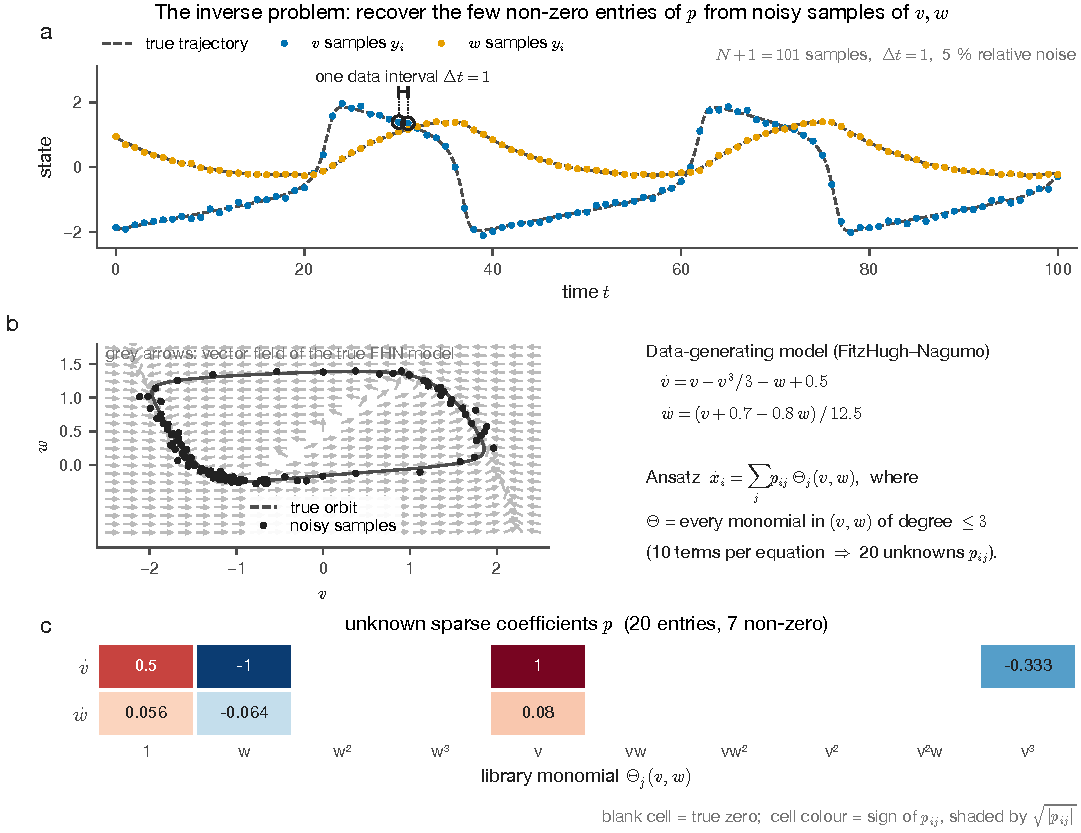
\includegraphics[width=\textwidth]{figures/fig01_problem.pdf}
\caption{\textbf{The inverse problem.} (a) The FHN states $v(t)$ (blue) and $w(t)$ (orange) with the $N=101$ noisy samples (dots) at spacing $\Delta t=1$; the thin dashed line is the exact trajectory. (b) Phase plane with the vector field (light arrows), the true orbit and the noisy samples. (c) The unknown $2\times10$ coefficient matrix over the monomial library $\{1,w,w^2,w^3,v,vw,vw^2,v^2,v^2w,v^3\}$: only 7 of 20 entries are non-zero (values shown). The task is to recover the non-zero pattern \emph{and} the values from the dots in (a). Data: \texttt{fhn\_data.csv}, \texttt{fhn\_fine.csv}, \texttt{fhn\_vector\_field.csv}, \texttt{fhn\_library.csv}.}\label{fig:01}\end{figure}

\begin{figure}[H]\centering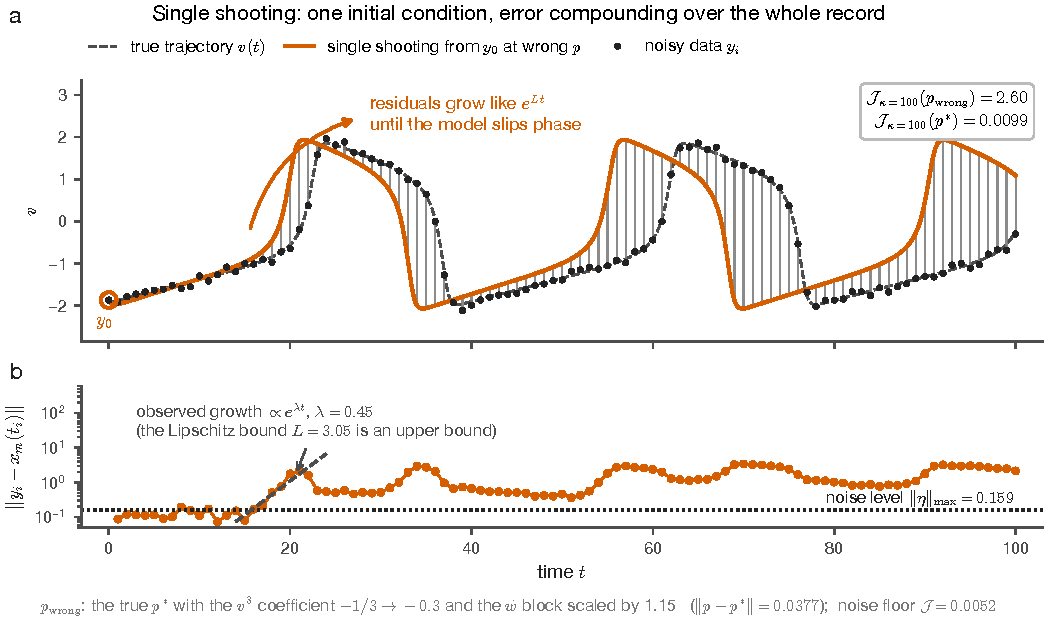
\includegraphics[width=\textwidth]{figures/fig02_single_shooting.pdf}
\caption{\textbf{Single shooting.} The model is integrated once from the first datum $y_0$ over the whole record with the wrong parameter $p_{\rm wrong}$ (vermilion); thin vertical lines are the residuals to the data. The residual (right, log scale) sits at the noise level until the model slips phase near $t\approx18$, then grows at an observed rate $\approx0.45$ per time unit (the Lipschitz bound $L=3.05$ is an upper bound, far above it) and saturates at the size of the attractor; the cost is $J_{100}(p_{\rm wrong})=2.60$ (vs $0.0099$ at $\pstar$), so a tiny parameter error produces a large, non-convex cost. Data: \texttt{concept\_segments.csv} (\texttt{param=wrong}, \texttt{window\_size=100}), \texttt{concept\_costs.csv}.}\label{fig:02}\end{figure}

\begin{figure}[H]\centering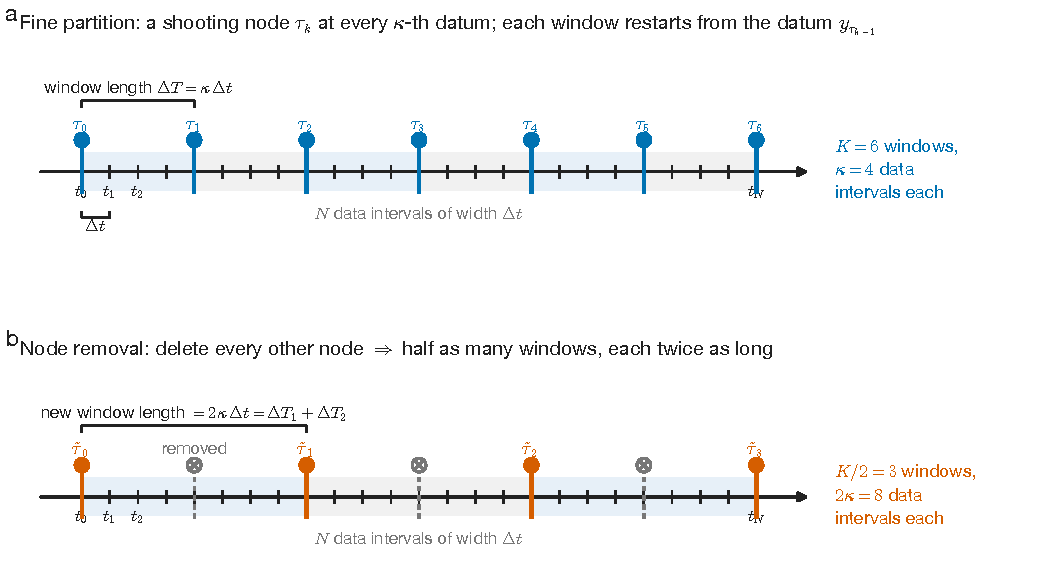
\includegraphics[width=\textwidth]{figures/fig03_partition.pdf}
\caption{\textbf{The shooting partition.} Top: the data times $t_0,\dots,t_N$ (ticks, spacing $\Delta t$) and the shooting nodes $\tau_0<\tau_1<\dots<\tau_K$ placed at every $\kappa$-th datum; the windows $[\tau_{k-1},\tau_k]$ of length $\Delta T=\kappa\Delta t$ are shaded alternately. Bottom: the coarser partition obtained by removing every other node ($K/2$ windows of length $2\Delta T$) --- the elementary step of guess propagation. Schematic (no data); replaces the manuscript's \texttt{shooting\_partition.png}.}\label{fig:03}\end{figure}

\begin{figure}[H]\centering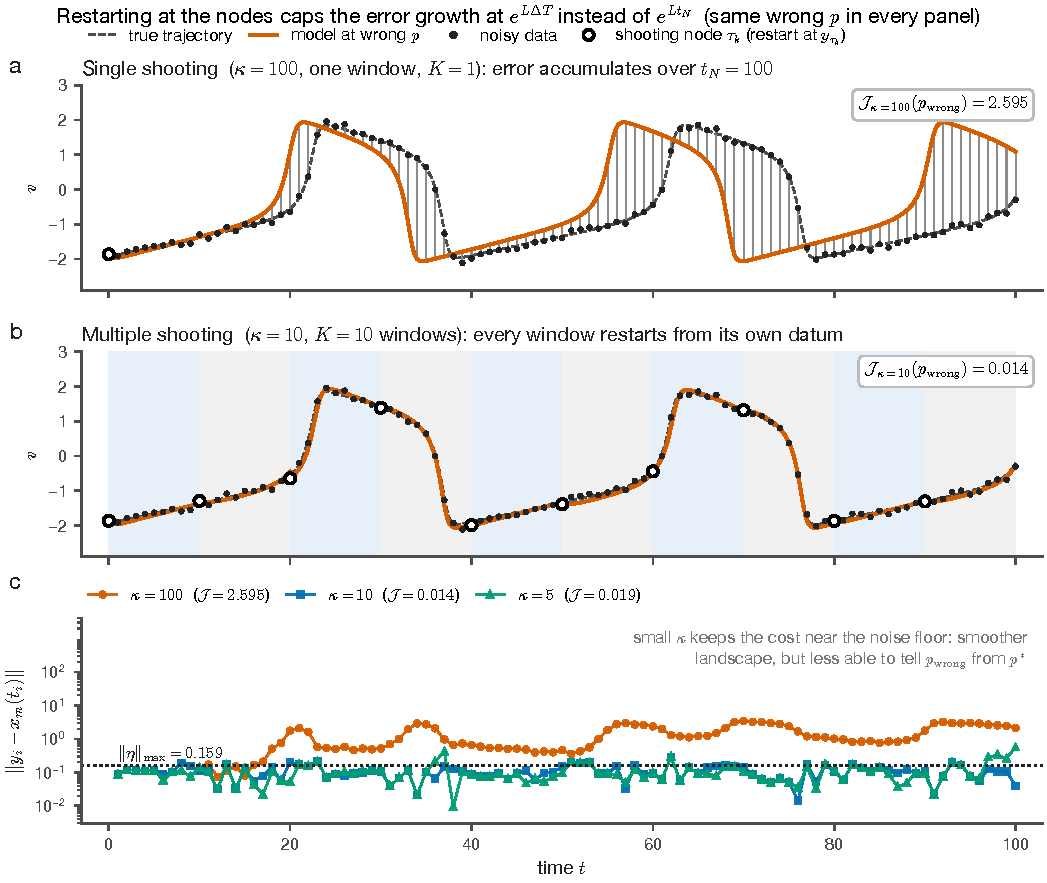
\includegraphics[width=\textwidth]{figures/fig04_multiple_shooting.pdf}
\caption{\textbf{Multiple shooting.} The same wrong parameter as \ref{fig:02}, integrated (a) as single shooting ($\kappa=100$, $J=2.60$) and (b) restarting from the datum at every 10th sample ($\kappa=10$, $J=0.0140$); windows are shaded, node markers highlighted, residual lines drawn to the data; (c) the per-datum residual magnitude on a log scale for $\kappa=100,10,5$ ($J=2.60,\,0.0140,\,0.0188$). Restarting resets the accumulated error at every node, so the exponential amplification is paid over $\Delta T=\kappa\Delta t$ instead of over the whole record; with $\kappa\le10$ the wrong model is only $1.4$--$1.8\times$ the cost of the true one, with $\kappa=100$ it is $260\times$. The flip side, visible in (c): short windows keep even a wrong model near the noise floor, i.e.\ they give a smooth landscape at the price of less power to discriminate $p$ from $\pstar$ --- which is why the sweep must end at single shooting. Replaces \texttt{multiple\_shooting.png}. Data: \texttt{concept\_segments.csv}, \texttt{concept\_costs.csv}.}\label{fig:04}\end{figure}

\begin{figure}[H]\centering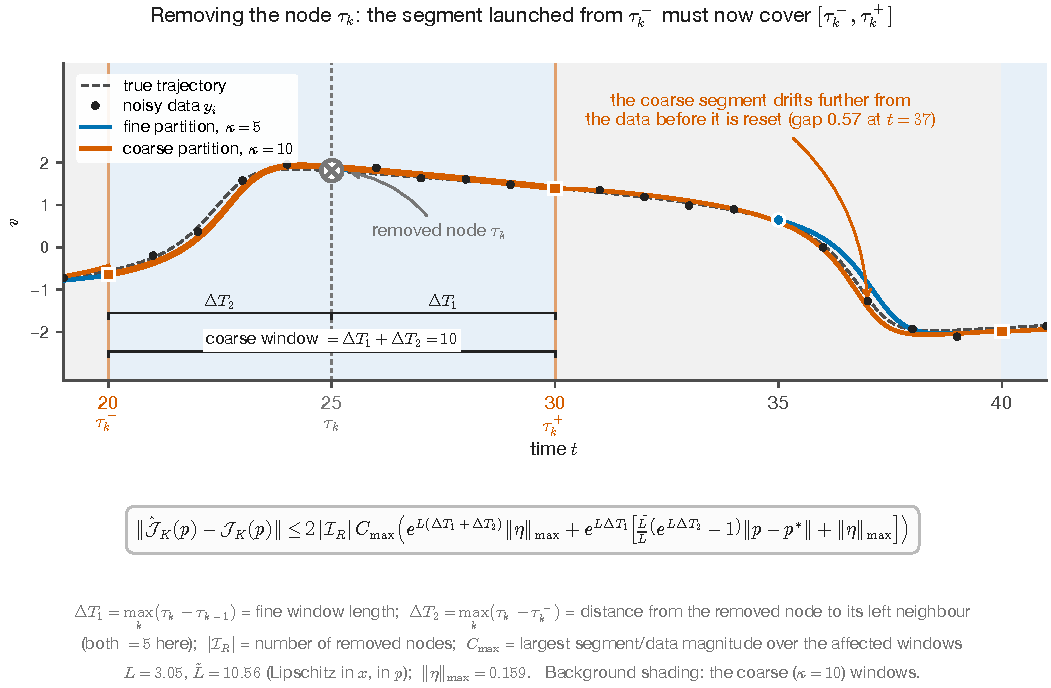
\includegraphics[width=\textwidth]{figures/fig05_node_removal.pdf}
\caption{\textbf{Node removal (Proposition~1).} Zoom on $t\in[19,41]$ with the wrong parameter: the fine partition ($\kappa=5$, blue segments) and the coarse one after removing the node $\tau_k$ at $t=25$ (open marker; $\kappa=10$, vermilion), with $\tau_k^-=20$ and $\tau_k^+=30$; the measured gap between the fine and coarse segments at $t=37$ is printed. After removal the segment launched at the left neighbour $\tau_k^-$ must cover $[\tau_k^-,\tau_k^+]$; the cost changes only on the windows adjacent to the removed nodes, by at most $2|I_R|\,C_{\max}\big(e^{L(\Delta T_1+\Delta T_2)}\lVert\eta\rVert_{\max}+e^{L\Delta T_1}[\tfrac{\tilde L}{L}(e^{L\Delta T_2}-1)\perr+\lVert\eta\rVert_{\max}]\big)$ with $\Delta T_1$ the fine window length and $\Delta T_2=\tau_k-\tau_k^-$. Design rule: remove few nodes at a time, prefer low-noise nodes, keep $\Delta T_2$ small. Replaces \texttt{comparison\_shooting\_nodes.png}.}\label{fig:05}\end{figure}

\begin{figure}[H]\centering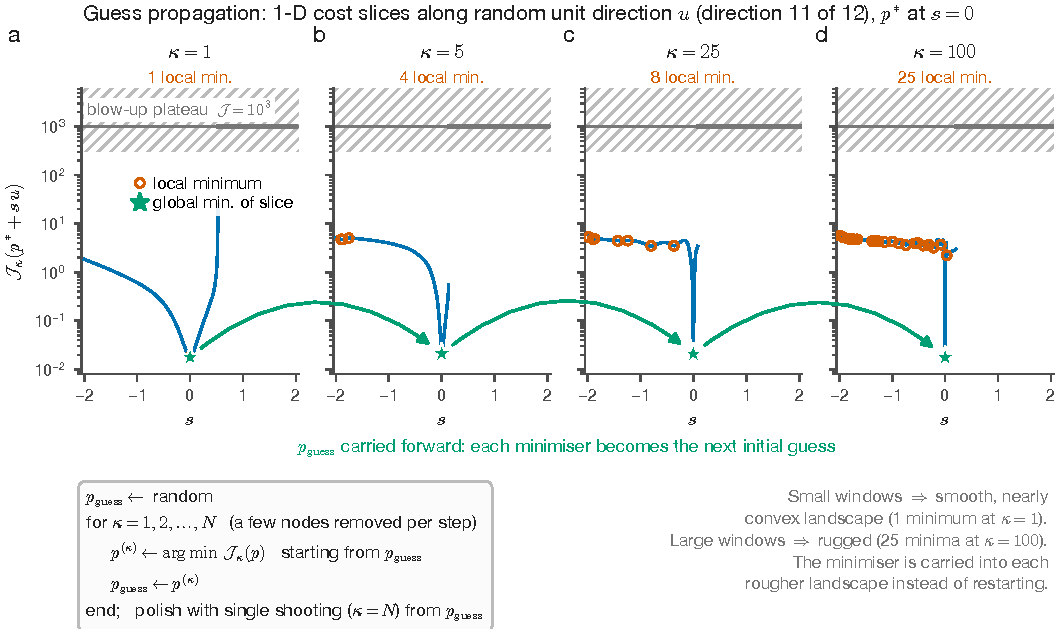
\includegraphics[width=\textwidth]{figures/fig06_guess_propagation.pdf}
\caption{\textbf{The guess-propagation algorithm.} One-dimensional slices $J_\kappa(\pstar+s\,u)$ along the same random unit direction $u$ (the one of the 12 directions of \ref{fig:13} with the most local minima at $\kappa=100$: 1, 4, 8, 25 local minima at $\kappa=1,5,25,100$, circled) for $\kappa=1,5,25,100$ (log scale; hatched band = blow-up plateau $J=10^3$; star = global minimum, which is at $s=0$ because the slices pass through $\pstar$). Small windows give a smooth, nearly convex landscape; large windows add local minima and a wide plateau. The algorithm solves the $\kappa=1$ problem from a random start and carries each minimiser (arrow) into the next, more rugged landscape, ending with a single-shooting polish. Data: \texttt{landscape\_1d\_slices.csv}.}\label{fig:06}\end{figure}

\begin{figure}[H]\centering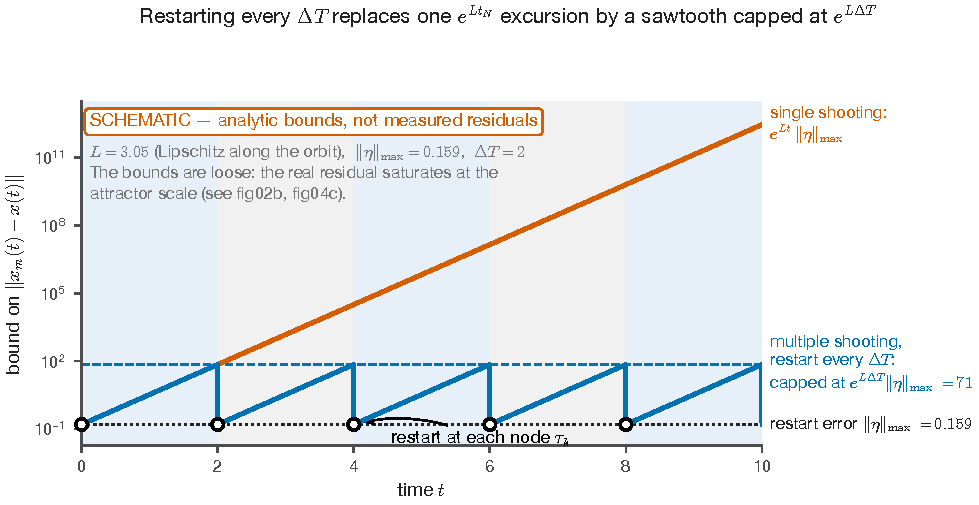
\includegraphics[width=0.75\textwidth]{figures/fig07_error_growth_schematic.pdf}
\caption{\textbf{Error growth, schematic.} The Lemma~1 envelope $e^{Lt}\lVert\eta\rVert_{\max}$ for single shooting (one restart at $t_0$) versus the sawtooth of multiple shooting, capped at $e^{L\Delta T}\lVert\eta\rVert_{\max}$ by the restart at every node, drawn with the report's $L=3.05$ and $\lVert\eta\rVert_{\max}=0.159$. This is the manuscript's one-line argument; \ref{fig:08} shows how loose the envelope is on the actual system.}\label{fig:07}\end{figure}

\section{Part B --- Numerical checks of the theory}\label{sec:theory}
\begin{figure}[H]\centering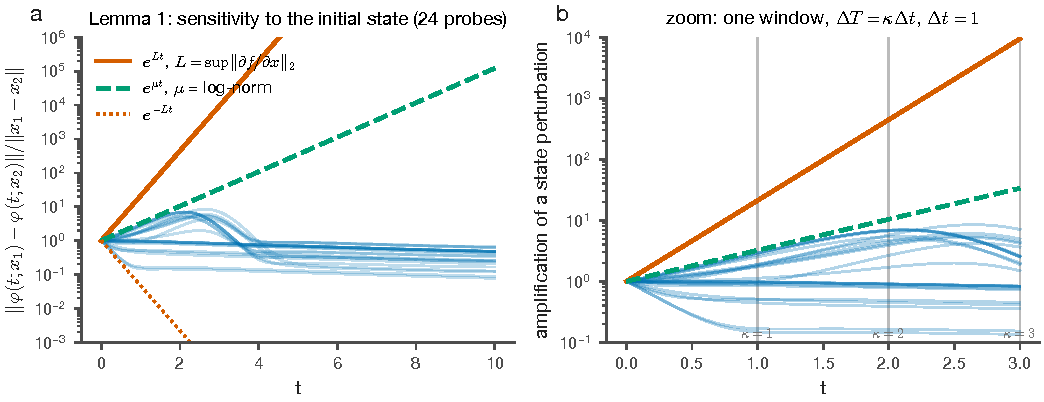
\includegraphics[width=\textwidth]{figures/fig08_lemma1_flow_sensitivity.pdf}
\caption{\textbf{Lemma~1 (flow sensitivity to the initial state).} Amplification $\lVert\varphi(t;\pstar,x_1)-\varphi(t;\pstar,x_2)\rVert/\lVert x_1-x_2\rVert$ for 24 probes ($x_1$ = a datum at 4 different phases of the orbit, $x_2=x_1+10^{-3}u$ for 6 random unit directions; blue), against $e^{Lt}$ with $L=\sup_{\rm orbit}\lVert\partial f/\partial x\rVert_2=3.05$ (vermilion), $e^{-Lt}$ (dotted) and $e^{\mu t}$ with the logarithmic norm $\mu=1.17$ (green dashed). (a) 10 time units, (b) zoom on the first three windows. The two-sided bound holds everywhere, but the actual amplification peaks at $\approx8$ near the fast jump of the relaxation oscillation and then \emph{contracts} (the limit cycle is attracting), whereas $e^{Lt}$ reaches $10^{13}$ at $t=10$. Data: \texttt{lemma1\_flow\_sensitivity.csv}, \texttt{concept\_meta.json}.}\label{fig:08}\end{figure}

\begin{figure}[H]\centering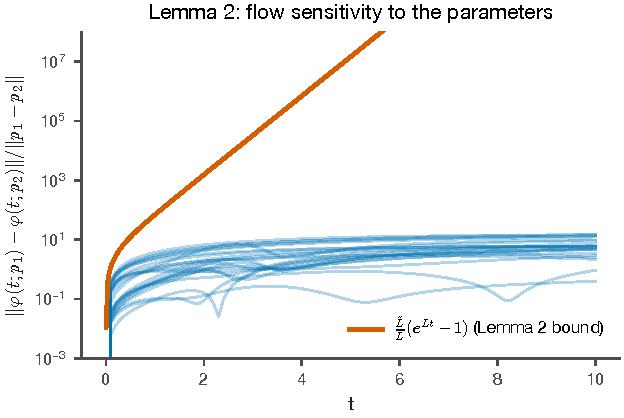
\includegraphics[width=0.62\textwidth]{figures/fig09_lemma2_param_sensitivity.pdf}
\caption{\textbf{Lemma~2 (flow sensitivity to the parameters).} $\lVert\varphi(t;p_1,x_0)-\varphi(t;p_2,x_0)\rVert/\lVert p_1-p_2\rVert$ for 24 probes ($p_2=\pstar+10^{-3}u$, random unit $u\in\mathbb R^{20}$) versus the bound $\tfrac{\tilde L}{L}(e^{Lt}-1)$ with $\tilde L=\sup_{\rm orbit}\lVert\partial f/\partial p\rVert_2=10.56$. The bound holds; the measured sensitivity saturates around $10$--$10^2$ because the orbit is attracting. Data: \texttt{lemma2\_param\_sensitivity.csv}.}\label{fig:09}\end{figure}

\begin{figure}[H]\centering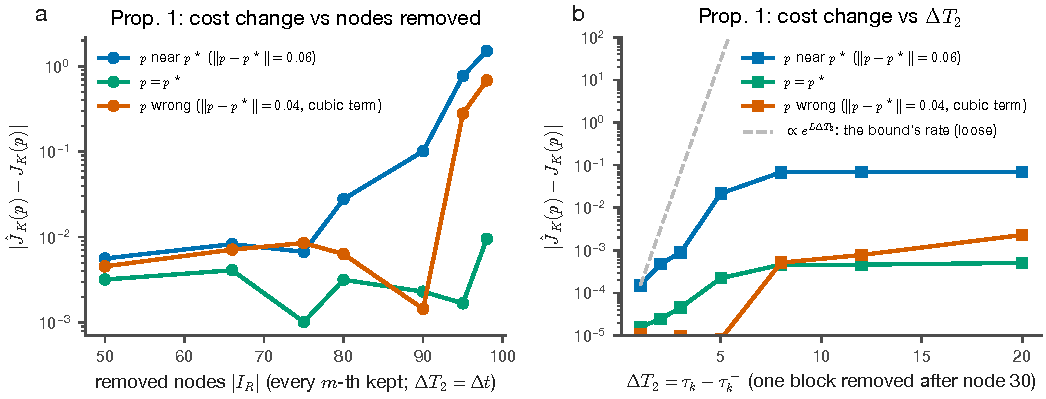
\includegraphics[width=\textwidth]{figures/fig10_prop1_node_removal.pdf}
\caption{\textbf{Proposition~1 (node removal changes the cost by a bounded amount).} Starting from the finest partition (every datum a node, $K=100$) with $\gamma=0$: (a) keep every $m$-th node so that $|I_R|=100-\lceil100/m\rceil$ nodes are removed ($\Delta T_2=\Delta t$ fixed, $\Delta T_1=m\Delta t$ grows), and (b) remove one contiguous block of $b$ nodes after node 30 ($|I_R|=b$, $\Delta T_2=b\Delta t$ grows). Shown for $p=\pstar$ (green), a vector $0.02$ away from $\pstar$ on 6 coefficients (blue, $\perr=0.06$) and $p_{\rm wrong}$ of Part~A (vermilion, $\perr=0.04$ concentrated on the cubic term). $|\hat J-J|$ grows with both $|I_R|$ and $\Delta T_2$, and much faster for the wrong parameter, as the proposition says; the bound's rate $e^{L\Delta T_2}$ (grey dashed in (b)) is far steeper than the observed growth, which saturates once the removed block spans a full fast excursion. Data: \texttt{prop1\_node\_removal.csv}.}\label{fig:10}\end{figure}

\section{Part C --- Cost landscapes}\label{sec:landscape}
\begin{figure}[H]\centering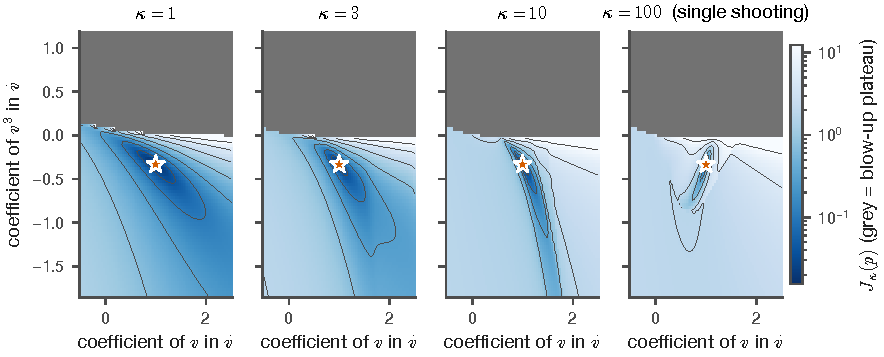
\includegraphics[width=\textwidth]{figures/fig11_landscape_2d_v_v3.pdf}
\caption{\textbf{2-D slices of $J_\kappa$ in the $(v,\,v^3)$ coefficient plane of the $\dot v$ equation.} All other coefficients at their true values, $x_0=y_0$, $\gamma=0.05$; star = truth $(1,-1/3)$; grey = blow-up plateau ($J\ge10^3$); colour is $\log J$. As $\kappa$ grows from 1 to 100 the basin around the truth narrows by an order of magnitude and the plateau expands: any positive cubic coefficient (above the horizontal edge) makes $\dot v\sim cv^3$ blow up in finite time, and at $\kappa=100$ even $v$-coefficients $>1.6$ do. This is the geometric reason the control arm fails at large $\kappa$. Data: \texttt{landscape\_2d\_v\_v3.csv}.}\label{fig:11}\end{figure}

\begin{figure}[H]\centering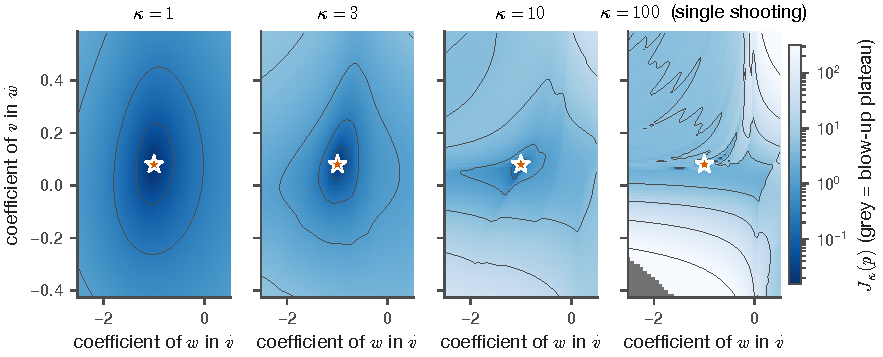
\includegraphics[width=\textwidth]{figures/fig12_landscape_2d_w_wv.pdf}
\caption{\textbf{2-D slices in the ($w$ in $\dot v$, $v$ in $\dot w$) plane.} Same protocol as \ref{fig:11}; star = truth $(-1,0.08)$. The $\dot w$ coefficient (vertical axis, true value 0.08) is a slow time-scale: at $\kappa=1$ the cost is almost flat along it (weakly identifiable from one-interval windows), and only long windows ($\kappa\ge10$) pin it down --- the mechanism behind the non-monotone parameter error along the sweep (\ref{fig:15}b). Data: \texttt{landscape\_2d\_w\_wv.csv}.}\label{fig:12}\end{figure}

\begin{figure}[H]\centering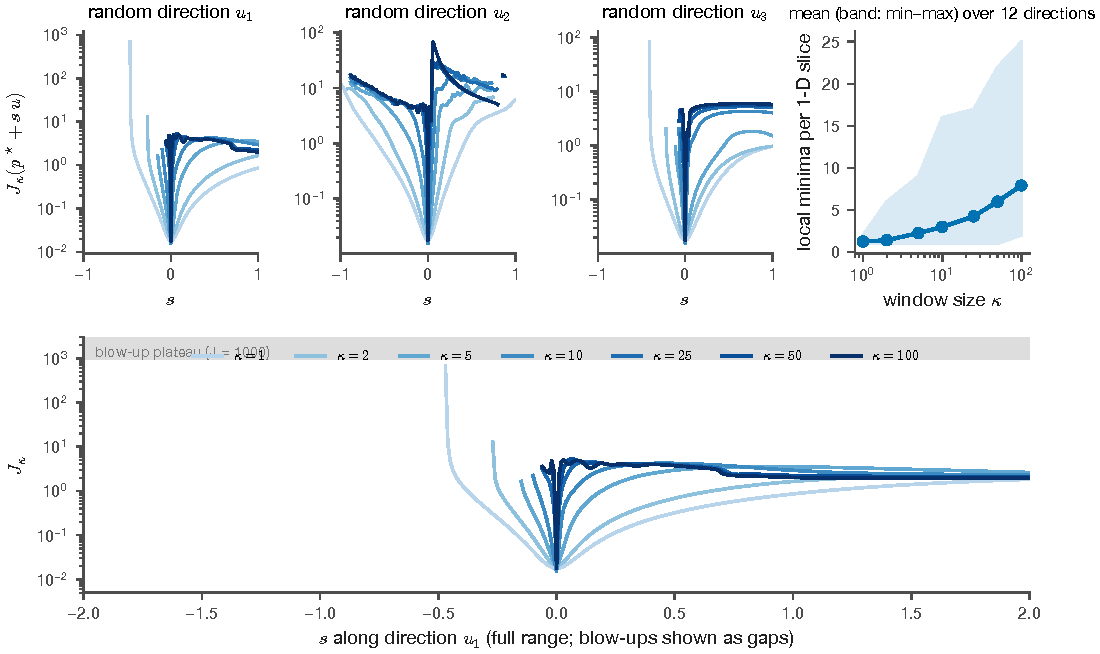
\includegraphics[width=\textwidth]{figures/fig13_landscape_1d_slices.pdf}
\caption{\textbf{1-D slices along random directions and the number of local minima.} Top row: $J_\kappa(\pstar+s\,u_d)$ for three random unit directions $u_d\in\mathbb R^{20}$ (colour light to dark = $\kappa=1,2,5,10,25,50,100$; gaps = plateau); top right: local minima per slice (mean over 12 directions, band = min--max) rising from $1.25$ at $\kappa=1$ to $7.9$ at $\kappa=100$. Bottom: the full $s\in[-2,2]$ range for direction 1. Larger windows sharpen the minimum (better conditioning \emph{at} the truth) but add spurious minima and cut the finite region down to $|s|\lesssim0.5$. Data: \texttt{landscape\_1d\_slices.csv}, \texttt{landscape\_1d\_minima.csv}.}\label{fig:13}\end{figure}

\begin{figure}[H]\centering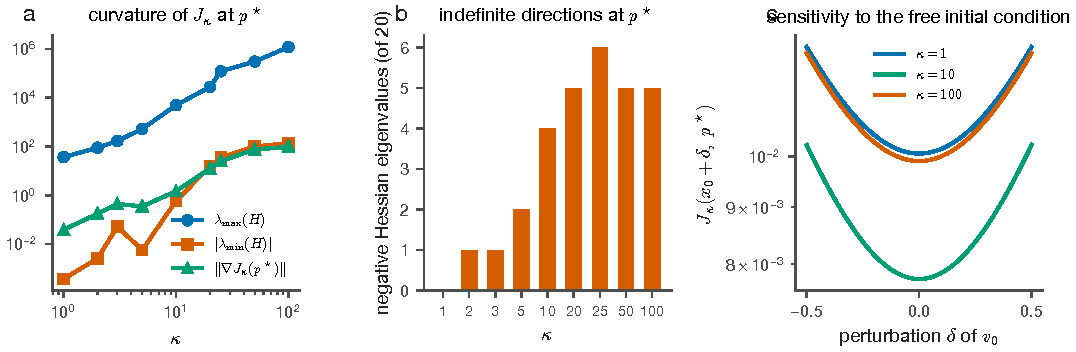
\includegraphics[width=\textwidth]{figures/fig14_hessian_conditioning.pdf}
\caption{\textbf{Curvature of the data term at $\pstar$ versus window size.} (a) Largest and smallest Hessian eigenvalues of the data term of $J_\kappa$ at $\pstar$ (ForwardDiff, 20 parameters) and the gradient norm: $\lambda_{\max}$ grows from $36$ ($\kappa=1$) to $1.2\times10^6$ ($\kappa=100$) while $\lVert\nabla J_\kappa(\pstar)\rVert$ grows from $0.04$ to $96$ --- with noisy data the truth is not a stationary point and drifts away from the minimiser as $\kappa$ grows. (b) The number of negative eigenvalues: the noisy cost is indefinite at $\pstar$ for every $\kappa\ge2$ (up to 6 of 20 directions), so the manuscript's strong-convexity assumption can only hold in a neighbourhood of the \emph{minimiser} $p^{(\kappa)}$, not of $\pstar$ (checked there in \ref{fig:37}). (c) Sensitivity of $J_\kappa$ to the free initial-condition variable $v_0$: a shallow parabola for every $\kappa$, because $x_0$ only enters through the first residual. Data: \texttt{hessian\_at\_ptrue.csv}, \texttt{landscape\_x0\_sensitivity.csv}.}\label{fig:14}\end{figure}

\section{Part D --- Guess propagation: the headline experiment}\label{sec:gp}
Protocol: 8 optimiser seeds $\times$ 3 arms $\times$ the 16-stage FULL schedule, Nelder--Mead with 2500 iterations per stage, $\gamma=0.05$, $S=10$, flat penalty. Table~\ref{tab:T1} gives the seed medians and the paired statistics per stage.

\begin{table}[H]\centering\scriptsize
\caption{Headline sweep, seed medians over 8 seeds (GP = guess propagation, best-GP = best-guess propagation, control = no propagation) and the paired difference GP $-$ control in $\perr$ with its 95\,\% bootstrap CI; ``\#GP better'' counts seeds where GP is strictly better; ``\#GP on plateau'' counts GP seeds whose minimiser is a blow-up (at $\kappa=1$ three seeds are on the plateau initially; two escape at $\kappa=2$ because the plateau at $\kappa=1$ is not flat for their simplex --- see text). Generated by \texttt{tables/make\_tables.py} from \texttt{sweeps.csv}.}\label{tab:T1}
\input{tables/T1_headline}
\end{table}

\begin{figure}[H]\centering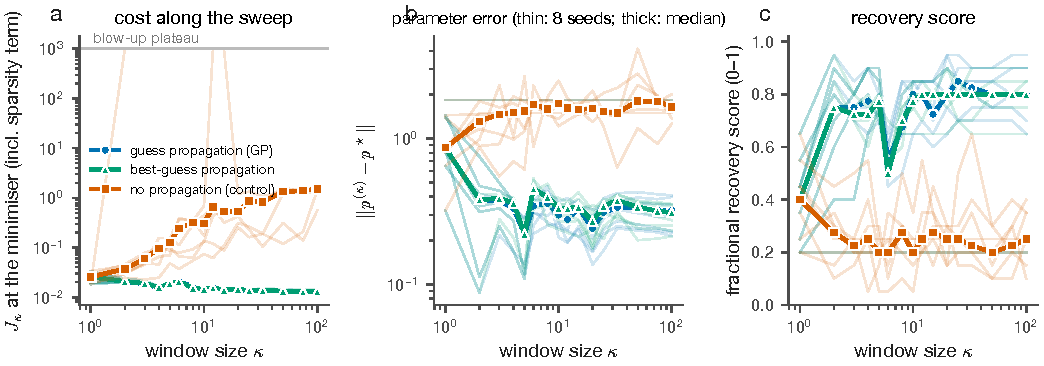
\includegraphics[width=\textwidth]{figures/fig15_sweep_headline.pdf}
\caption{\textbf{Guess propagation versus no propagation, 8 seeds.} (a) Cost, (b) parameter error and (c) recovery score at the minimiser of each stage; thin lines = individual seeds, thick = median; blue circles GP, green triangles best-GP, vermilion squares control. All arms coincide at $\kappa=1$ (same start). From $\kappa=2$ on, GP drops to $\perr\approx0.22$--$0.38$ and ends single shooting at $0.32$ (score $0.80$), whereas the control climbs back to the seed distance ($1.65$ at $\kappa=100$; 25\,\% of its seeds end on the plateau, all others in spurious minima with $J$ up to $1.5$). One GP seed (seed 1) starts on the plateau at $\kappa=1$ and never moves (flat line at $1.84$). The parameter error is \emph{not} monotone: it is smallest at $\kappa=5$ ($0.22$) and drifts up to $0.32$ while the cost keeps falling --- the noise-induced bias of \ref{fig:14}. Data: \texttt{sweeps.csv} (\texttt{exp=main}).}\label{fig:15}\end{figure}

\begin{figure}[H]\centering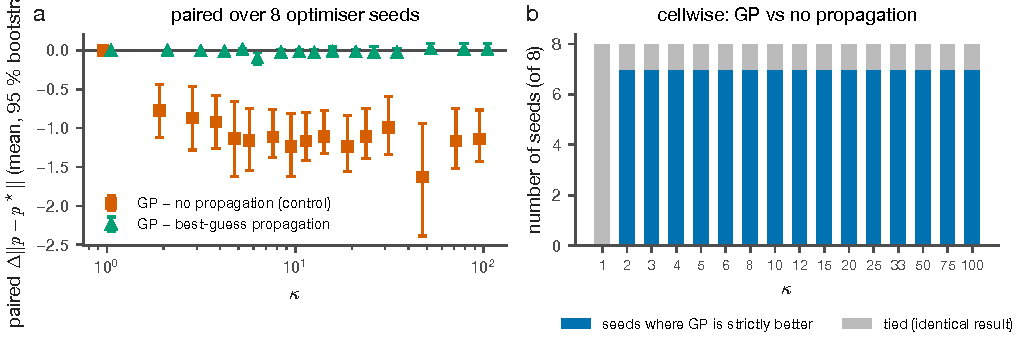
\includegraphics[width=\textwidth]{figures/fig16_sweep_paired.pdf}
\caption{\textbf{Paired comparison.} (a) Mean paired difference in $\perr$ (GP minus control, vermilion squares; GP minus best-GP, green triangles) with 95\,\% bootstrap CIs over the 8 seeds; the GP--control difference is $-0.77$ at $\kappa=2$, $-1.14$ $[-1.43,-0.77]$ at $\kappa=100$, and its CI excludes zero at every $\kappa\ge2$; GP and best-GP are statistically indistinguishable. (b) Cellwise counts: GP is strictly better than the control in 7 of 8 seeds at every $\kappa\ge2$ and tied in the eighth (the plateau seed). Data: \texttt{derived\_paired\_main.csv}.}\label{fig:16}\end{figure}

\begin{figure}[H]\centering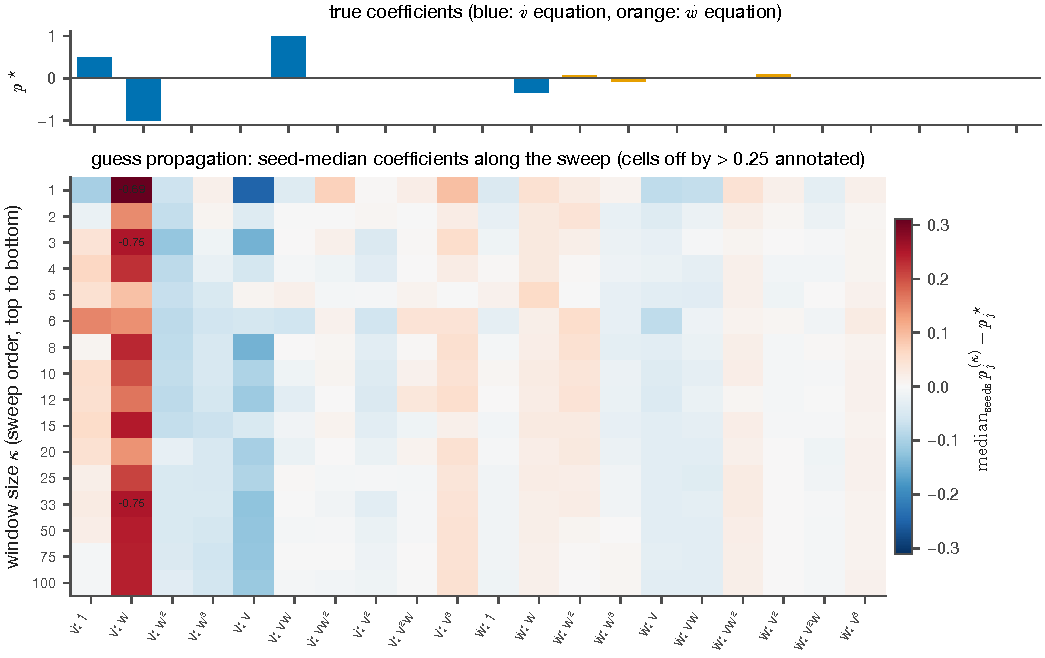
\includegraphics[width=\textwidth]{figures/fig17_sweep_coefficients.pdf}
\caption{\textbf{Which coefficients are recovered when.} Top: the true coefficients (library order, $\dot v$ block blue, $\dot w$ block orange). Bottom: seed-median GP coefficient minus truth for every stage of the sweep (rows) and every coefficient (columns), diverging colour scale. The $v$ and constant coefficients of $\dot v$ are right within $0.1$ from $\kappa=2$; the $w$ coefficient of $\dot v$ stays $\approx0.3$ too small at every $\kappa$ and the $v$ coefficient $\approx0.1$ too small --- the shrinkage of the smooth-$\ell_1$ term at $\gamma=0.05$ (cf.~\ref{fig:24}, where $\gamma=0.01$ removes the shrinkage but loses sparsity); the slow $\dot w$ coefficients ($\le0.08$ in magnitude) are within $0.05$. Data: \texttt{sweep\_minimizers.csv}.}\label{fig:17}\end{figure}

\begin{figure}[H]\centering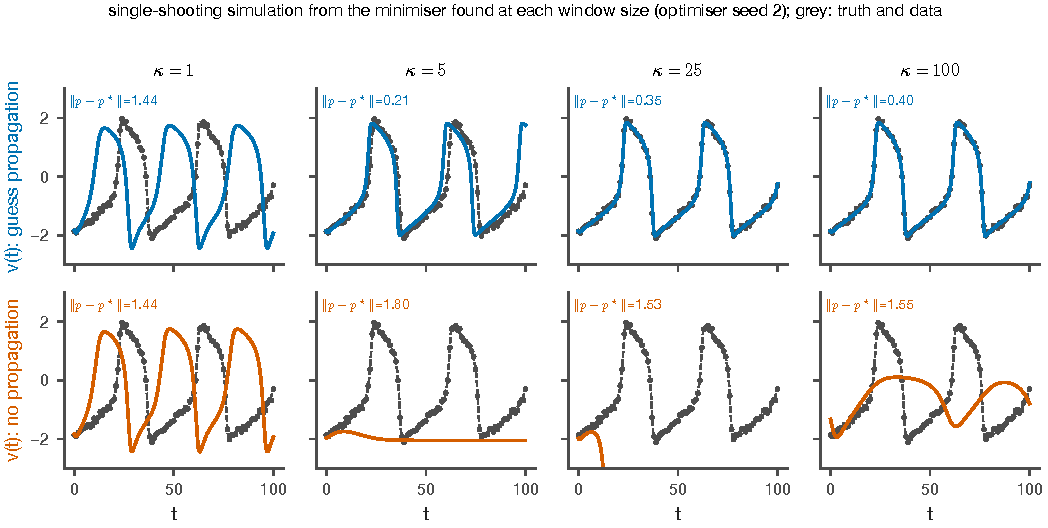
\includegraphics[width=\textwidth]{figures/fig18_sweep_filmstrip.pdf}
\caption{\textbf{Filmstrip of the sweep (seed 2).} Single-shooting simulation of $v(t)$ from the minimiser returned at $\kappa=1,5,25,100$ (columns) for GP (top, blue) and the control (bottom, vermilion); grey dashed = truth, dots = data; the parameter error is printed in each panel. The GP fit tracks the data at every stage; the control loses the trajectory as soon as the windows are long. Frames of \texttt{figures/anim\_sweep.gif}. Data: \texttt{sweep\_fits.csv}, \texttt{sweeps.csv}.}\label{fig:18}\end{figure}

\begin{figure}[H]\centering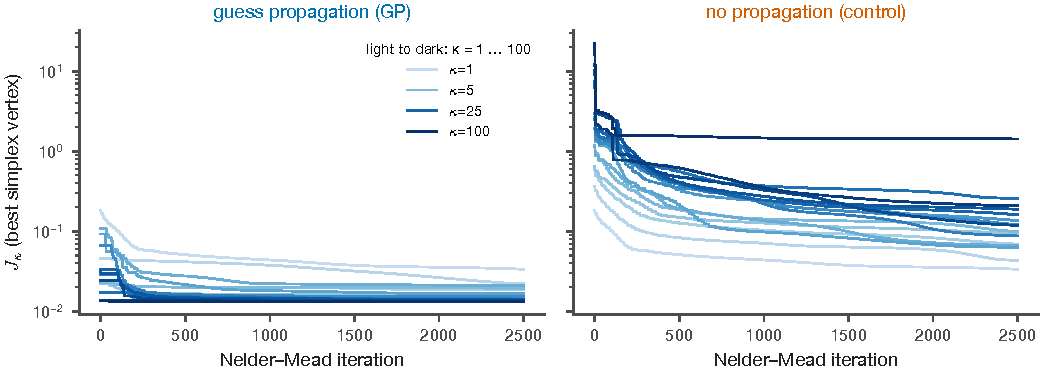
\includegraphics[width=\textwidth]{figures/fig19_sweep_traces.pdf}
\caption{\textbf{Optimiser traces (seed 2).} Best simplex value of Nelder--Mead versus iteration for every stage (colour light to dark = $\kappa=1\dots100$), GP (left) and control (right). With propagation each stage starts within a factor of a few of its final cost and converges; without it every stage starts from the same distant seed and, for $\kappa\ge10$, from the plateau (flat traces at $10^3$) or a spurious minimum. Data: \texttt{traces\_seed2.csv}.}\label{fig:19}\end{figure}

\begin{figure}[H]\centering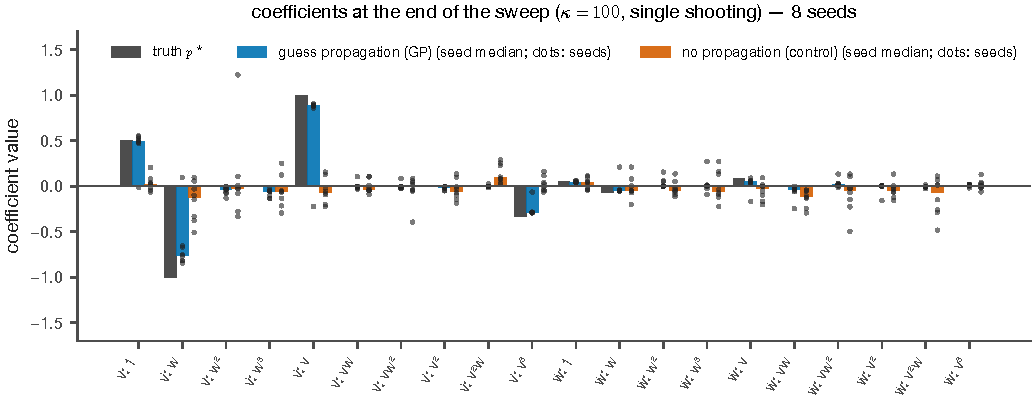
\includegraphics[width=\textwidth]{figures/fig20_final_coefficients.pdf}
\caption{\textbf{Coefficients at the end of the sweep ($\kappa=100$).} Truth (grey), GP seed-median (blue) and control seed-median (vermilion) with the 8 individual seeds as dots, correctly labelled in the library order (the repository's bar-chart labels encoded the pre-refactor order --- fix N1, \S\ref{sec:bugs}). GP recovers the support (7 non-zeros, no false positive in the median) with the shrinkage noted in \ref{fig:17}; the control's median is near zero everywhere because its seeds scatter. Data: \texttt{sweep\_minimizers.csv}.}\label{fig:20}\end{figure}

\paragraph{Three GP seeds on the plateau at $\kappa=1$, one forever.} Table~\ref{tab:T1} shows 3 GP seeds with a blow-up minimiser at $\kappa=1$ but only 1 from $\kappa=2$ on. A random start with a positive cubic coefficient of order $0.1$--$0.3$ blows up within one time unit ($\dot v\sim cv^3$, $|v|\approx2$), so the loss is $10^3$ at the start; if the whole initial Nelder--Mead simplex sits on the plateau the optimiser declares convergence after 0 iterations (all vertices equal) and returns the seed. Two of the three starts have a simplex vertex off the plateau at $\kappa=2$ and escape; seed 1 does not, at any $\kappa$. This is a property of the \emph{flat} penalty, not of guess propagation; the graded penalty (\ref{fig:22}, \ref{fig:28}) removes it.

\section{Part E --- Variations}\label{sec:var}
Table~\ref{tab:T2} lists the end-of-sweep ($\kappa=100$) seed medians of every variation arm; each figure below shows the whole sweep.

\begin{table}[H]\centering\scriptsize
\caption{End-of-sweep ($\kappa=100$) seed medians for every variation arm: $\perr$, recovery score, fraction of seeds on the plateau, and median wall time per stage. Arms within an experiment share seeds and schedule (SHORT for noise/sparsity/iters/substeps/seedscale, FULL for schedule/penalty/optimizer). ``seedscale'' arms are named \texttt{sc<scale>\_<mode>\_<penalty>}. Generated from \texttt{sweeps.csv}.}\label{tab:T2}
\begin{tabular}{lrrrrrr}
\toprule
experiment & arm & n\_seeds & $\|p-p^\star\|$ ($\kappa$=100) & score & plateau frac & wall s per $\kappa$ \\
\midrule
schedule & coarse & 8 & 0.5239 & 0.55 & 0.125 & 2.069 \\
schedule & dense & 8 & 0.3015 & 0.8 & 0.125 & 2.072 \\
schedule & jump & 8 & 0.7635 & 0.425 & 0.125 & 2.098 \\
penalty & propagate\_graded & 8 & 0.274 & 0.825 & 0 & 2.107 \\
penalty & reset\_graded & 8 & 1.631 & 0.3 & 0 & 1.88 \\
noise & propagate $\sigma$=0.0 & 6 & 0.2313 & 0.8 & 0.1667 & 2.058 \\
noise & propagate $\sigma$=0.01 & 6 & 0.3617 & 0.7 & 0.1667 & 2.117 \\
noise & propagate $\sigma$=0.02 & 6 & 0.2482 & 0.875 & 0.1667 & 2.102 \\
noise & propagate $\sigma$=0.05 & 6 & 0.2217 & 0.8 & 0.1667 & 2.087 \\
noise & propagate $\sigma$=0.1 & 6 & 0.3135 & 0.625 & 0.1667 & 2.049 \\
noise & propagate $\sigma$=0.2 & 6 & 1.881 & 0.225 & 0.1667 & 2.134 \\
noise & reset $\sigma$=0.0 & 6 & 1.633 & 0.25 & 0.3333 & 1.845 \\
noise & reset $\sigma$=0.01 & 6 & 1.602 & 0.2 & 0.3333 & 1.878 \\
noise & reset $\sigma$=0.02 & 6 & 1.669 & 0.225 & 0.3333 & 1.876 \\
noise & reset $\sigma$=0.05 & 6 & 1.649 & 0.25 & 0.3333 & 1.867 \\
noise & reset $\sigma$=0.1 & 6 & 1.679 & 0.225 & 0.3333 & 1.847 \\
noise & reset $\sigma$=0.2 & 6 & 1.702 & 0.2 & 0.3333 & 1.849 \\
sparsity & 0.0 & 6 & 0.8142 & 0.375 & 0.1667 & 2.175 \\
sparsity & 0.001 & 6 & 0.8433 & 0.475 & 0.1667 & 2.21 \\
sparsity & 0.01 & 6 & 0.8875 & 0.525 & 0.1667 & 2.085 \\
sparsity & 0.05 & 6 & 0.2217 & 0.8 & 0.1667 & 2.051 \\
sparsity & 0.2 & 6 & 0.4741 & 0.65 & 0.1667 & 2.033 \\
sparsity & 1.0 & 6 & 1.01 & 0.6 & 0.1667 & 2.003 \\
optimizer & bfgs\_propagate & 8 & 0.2053 & 0.95 & 0.125 & 1.439 \\
optimizer & bfgs\_reset & 8 & 1.648 & 0.225 & 0.625 & 13.55 \\
optimizer & lbfgs\_propagate & 8 & 0.2053 & 0.95 & 0.125 & 102.4 \\
optimizer & lbfgs\_reset & 8 & 1.648 & 0.225 & 0.625 & 15.25 \\
iters & 250 & 4 & 1.722 & 0.325 & 0.25 & 0.431 \\
iters & 500 & 4 & 1.426 & 0.2 & 0.25 & 0.8172 \\
iters & 1000 & 4 & 0.6087 & 0.575 & 0.25 & 1.047 \\
iters & 2500 & 4 & 0.2658 & 0.775 & 0.25 & 2.014 \\
iters & 5000 & 4 & 0.1986 & 0.9 & 0.25 & 3.867 \\
substeps & 1 & 4 & 0.4988 & 0.75 & 0 & 0.2064 \\
substeps & 2 & 4 & 0.3377 & 0.675 & 0.25 & 0.4289 \\
substeps & 5 & 4 & 0.2853 & 0.825 & 0.25 & 1.027 \\
substeps & 10 & 4 & 0.2658 & 0.775 & 0.25 & 1.991 \\
substeps & 20 & 4 & 0.2658 & 0.775 & 0.25 & 4.059 \\
seedscale & sc0.01\_propagate\_flat & 8 & 0.1967 & 0.85 & 0 & 2.064 \\
seedscale & sc0.01\_propagate\_graded & 8 & 0.1967 & 0.85 & 0 & 2.062 \\
seedscale & sc0.01\_reset\_flat & 8 & 1.65 & 0.35 & 0.125 & 1.951 \\
seedscale & sc0.01\_reset\_graded & 8 & 1.589 & 0.375 & 0 & 1.88 \\
seedscale & sc0.03\_propagate\_flat & 8 & 0.2857 & 0.775 & 0 & 2.085 \\
seedscale & sc0.03\_propagate\_graded & 8 & 0.2857 & 0.775 & 0 & 2.084 \\
seedscale & sc0.03\_reset\_flat & 8 & 1.586 & 0.475 & 0.25 & 1.875 \\
seedscale & sc0.03\_reset\_graded & 8 & 1.573 & 0.35 & 0 & 1.934 \\
seedscale & sc0.1\_propagate\_flat & 8 & 0.2086 & 0.85 & 0.125 & 2.025 \\
seedscale & sc0.1\_propagate\_graded & 8 & 0.2086 & 0.85 & 0 & 2.047 \\
seedscale & sc0.1\_reset\_flat & 8 & 1.649 & 0.25 & 0.25 & 1.888 \\
seedscale & sc0.1\_reset\_graded & 8 & 1.631 & 0.3 & 0 & 1.864 \\
seedscale & sc0.3\_propagate\_flat & 8 & 0.4237 & 0.7 & 0.25 & 2.043 \\
seedscale & sc0.3\_propagate\_graded & 8 & 0.3495 & 0.825 & 0.125 & 2.179 \\
seedscale & sc0.3\_reset\_flat & 8 & 2.443 & 0.1 & 0.25 & 1.875 \\
seedscale & sc0.3\_reset\_graded & 8 & 2.702 & 0.1 & 0.25 & 1.831 \\
\bottomrule
\end{tabular}

\end{table}

\begin{figure}[H]\centering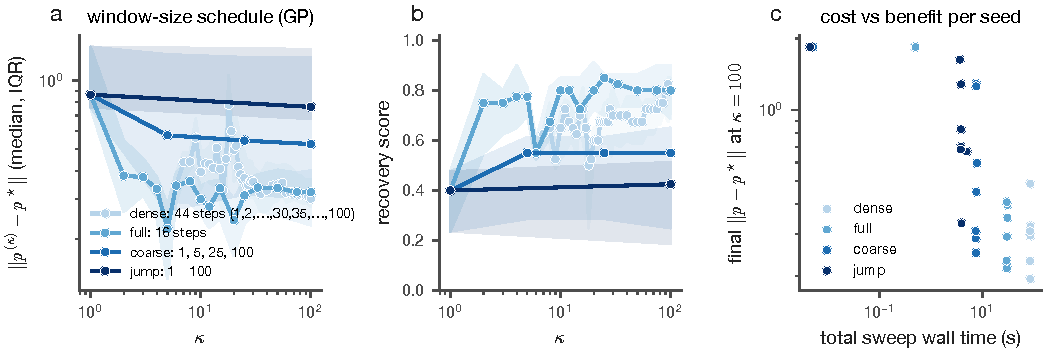
\includegraphics[width=\textwidth]{figures/fig21_schedule.pdf}
\caption{\textbf{Window-size schedule (how many nodes to remove per step).} GP with the DENSE (44 stages), FULL (16), COARSE (4) and JUMP (2: $\kappa=1$ then 100) schedules, 8 seeds each: (a) $\perr$ and (b) score along the sweep (median, IQR band), (c) final error against total wall time per seed. Final medians: dense $0.30$, full $0.32$, coarse $0.52$, jump $0.76$ (scores $0.80,0.80,0.55,0.43$). Removing few nodes per step is what makes propagation work --- the manuscript's design rule --- and the dense schedule costs $2.7\times$ the time of the full one for no gain. Data: \texttt{sweeps.csv} (\texttt{exp=schedule}, \texttt{main/propagate}).}\label{fig:21}\end{figure}

\begin{figure}[H]\centering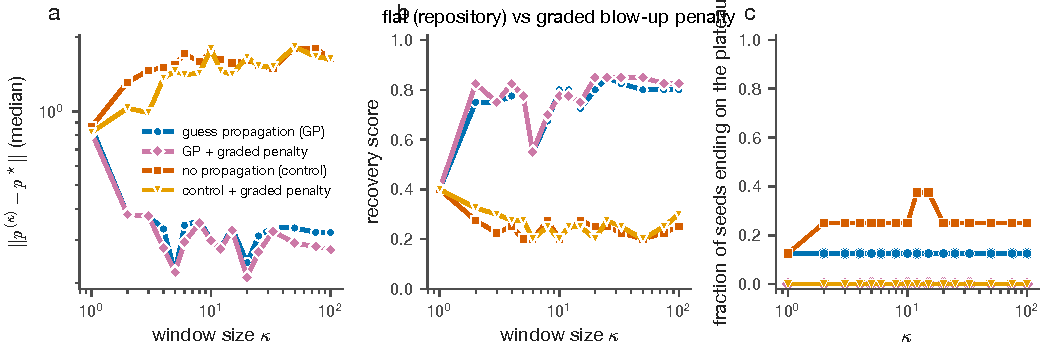
\includegraphics[width=\textwidth]{figures/fig22_penalty.pdf}
\caption{\textbf{Flat versus graded blow-up penalty.} The repository returns the constant $10^3$ on blow-up; the graded variant adds a term that decreases with the index at which the blow-up occurred. GP with the graded penalty (purple) ends at $\perr=0.27$, score $0.83$, with \emph{no} seed on the plateau at any stage (c), versus $0.32$ / $0.80$ / 12.5\,\% for the flat penalty (blue): seed 1 is rescued. For the control the penalty changes nothing (still $\approx1.6$): without propagation the failure is the landscape, not the plateau. Data: \texttt{sweeps.csv} (\texttt{exp=penalty}, \texttt{main}).}\label{fig:22}\end{figure}

\begin{figure}[H]\centering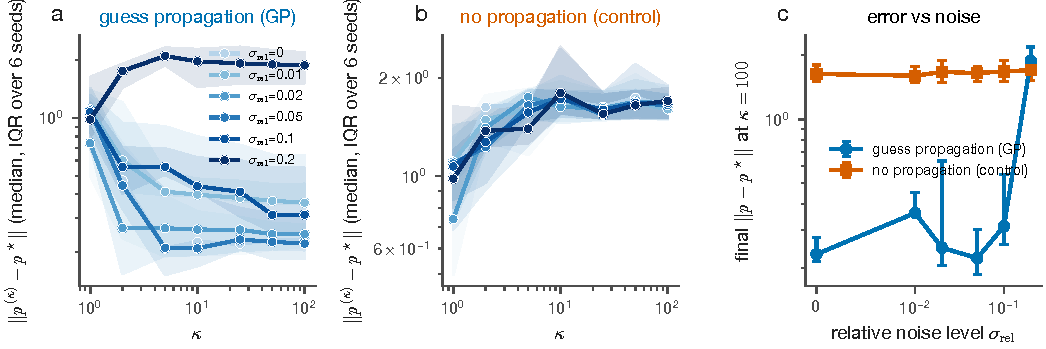
\includegraphics[width=\textwidth]{figures/fig23_noise.pdf}
\caption{\textbf{Observation noise.} GP (a) and control (b) along the SHORT schedule for relative noise $\sigma_{\rm rel}\in\{0,0.01,0.02,0.05,0.1,0.2\}$ (6 seeds each; the data-noise seed is fixed so the noise realisations are scaled versions of one another); (c) final error at $\kappa=100$. GP ends at $0.22$--$0.36$ for $\sigma_{\rm rel}\le0.1$ and fails at $0.2$ ($1.88$); the control ends at $1.6$--$1.7$ at \emph{every} noise level including $0$ --- restarting from the seed fails because of the landscape, not the noise. Note that the GP error does not go to zero at zero noise ($0.23$): the remaining error is the sparsity-term shrinkage and Nelder--Mead's finite accuracy, not noise. Data: \texttt{sweeps.csv} (\texttt{exp=noise}).}\label{fig:23}\end{figure}

\begin{figure}[H]\centering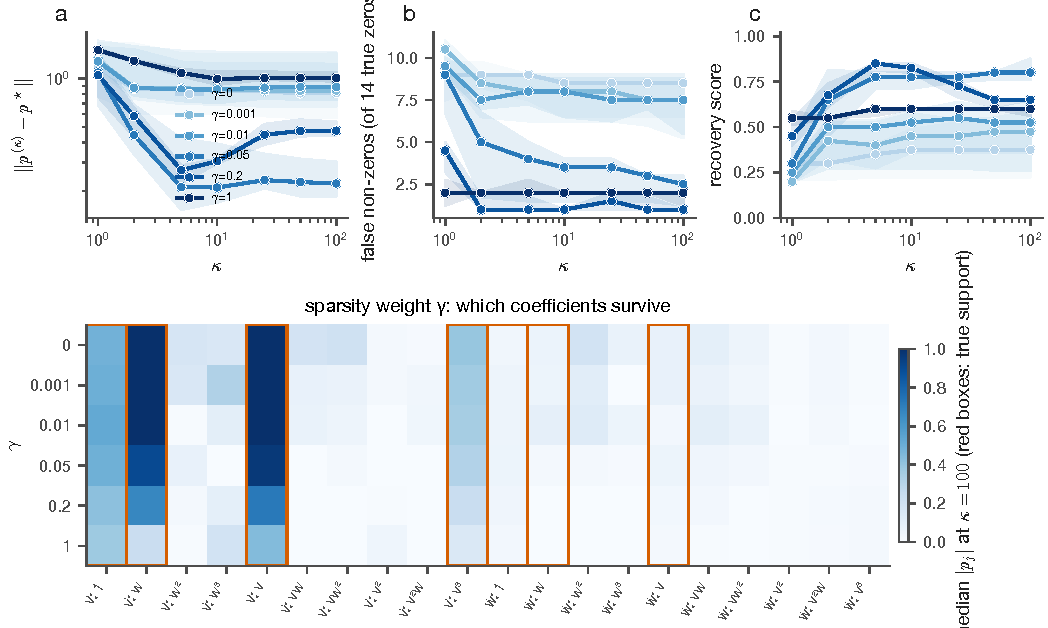
\includegraphics[width=\textwidth]{figures/fig24_sparsity.pdf}
\caption{\textbf{Sparsity weight $\gamma$.} GP along the SHORT schedule for $\gamma\in\{0,10^{-3},10^{-2},0.05,0.2,1\}$, 6 seeds: (a) $\perr$, (b) false non-zeros, (c) score; bottom: median $|p_j|$ at $\kappa=100$ per coefficient (red boxes = true support). $\gamma=0.05$ (the repository default) is the best of the six ($0.22$, score $0.80$); with $\gamma\le0.01$ the Nelder--Mead sweep wanders into dense, wrong models ($0.81$--$0.89$, 4--6 false non-zeros), and $\gamma\ge0.2$ over-shrinks the true coefficients ($0.47$, $1.01$). Data: \texttt{sweeps.csv}, \texttt{sweep\_minimizers.csv} (\texttt{exp=sparsity}).}\label{fig:24}\end{figure}

\begin{figure}[H]\centering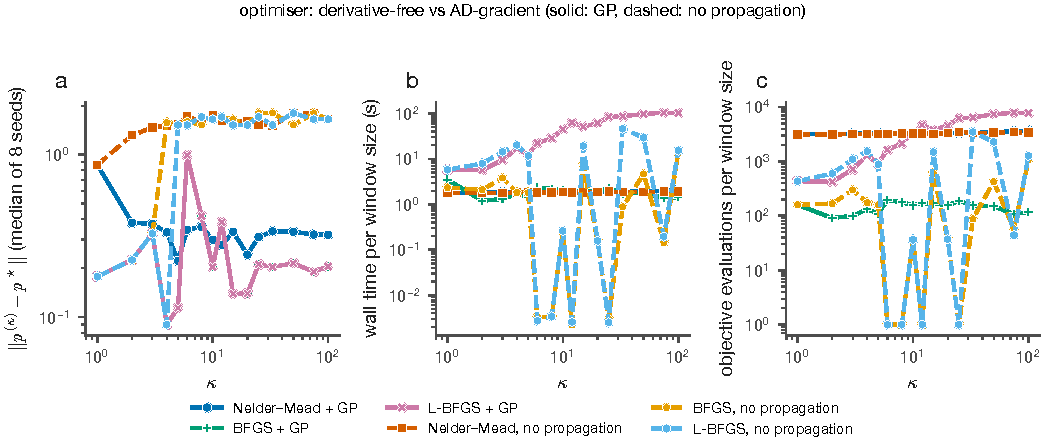
\includegraphics[width=\textwidth]{figures/fig25_optimizers.pdf}
\caption{\textbf{Optimiser: derivative-free versus AD gradient.} Nelder--Mead, BFGS and L-BFGS (exact ForwardDiff gradient of the windowed loss, possible after fix F4), with (solid) and without (dashed) propagation, 8 seeds, FULL schedule: (a) median $\perr$, (b) wall time per stage, (c) objective evaluations per stage. BFGS+GP is the best arm ($0.21$, score $0.95$) and needs $\approx150$ evaluations per stage instead of $3500$; L-BFGS reaches the same minimiser but hits the iteration cap at large $\kappa$ ($100$\,s per stage). Without propagation the gradient methods stop after one evaluation whenever the start is on the plateau (zero gradient) --- 62--71\,\% of their stages --- and otherwise converge to spurious minima. Data: \texttt{sweeps.csv} (\texttt{exp=optimizer}, \texttt{main}).}\label{fig:25}\end{figure}

\begin{figure}[H]\centering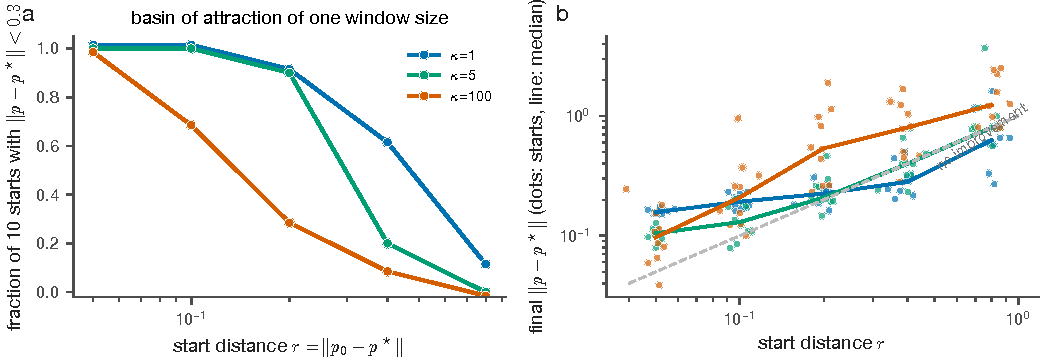
\includegraphics[width=\textwidth]{figures/fig26_basin.pdf}
\caption{\textbf{Basin of attraction of a single window size.} One Nelder--Mead run (2500 iterations) of $J_\kappa$ from $p_0=\pstar+r\,u$ (10 random unit directions per radius $r\in\{0.05,\dots,0.8\}$) for $\kappa=1,5,100$: (a) fraction of starts ending within $0.3$ of $\pstar$, (b) final error (dots) and median. Single shooting ($\kappa=100$) only converges from $r\le0.1$; $\kappa=5$ from $r\le0.2$; $\kappa=1$ never gets below $\approx0.15$ (its noise/shrinkage floor) but improves every start up to $r=0.4$. This is the quantitative version of \ref{fig:06}: small windows have the wide basin, large windows have the accurate minimum. Data: \texttt{sweeps.csv} (\texttt{exp=basin}).}\label{fig:26}\end{figure}

\begin{figure}[H]\centering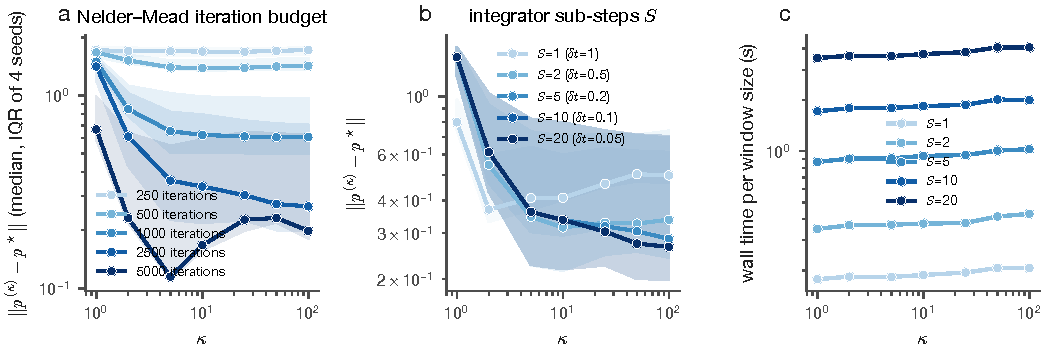
\includegraphics[width=\textwidth]{figures/fig27_iters_substeps.pdf}
\caption{\textbf{Iteration budget and integrator resolution.} (a) GP with 250--5000 Nelder--Mead iterations per stage (4 seeds, SHORT): final medians $1.72,1.43,0.61,0.27,0.20$ --- fewer than 2500 iterations in 22 dimensions is not converged; (b) sub-steps $S\in\{1,2,5,10,20\}$ per data interval ($\delta t=1/S$): $S\ge5$ gives the same answer ($0.27$--$0.29$), $S=1$ ($\delta t=\Delta t$) biases the fit ($0.50$) but never blows up; (c) wall time scales linearly with $S$. Data: \texttt{sweeps.csv} (\texttt{exp=iters}, \texttt{exp=substeps}).}\label{fig:27}\end{figure}

\begin{figure}[H]\centering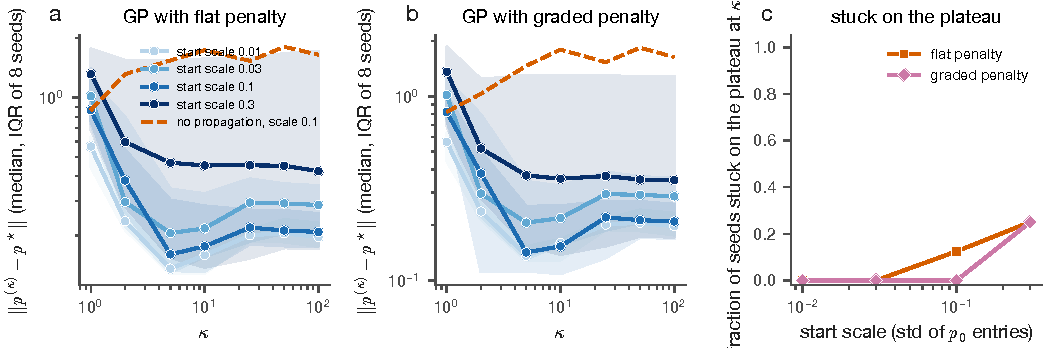
\includegraphics[width=\textwidth]{figures/fig28_seedscale.pdf}
\caption{\textbf{Start distance.} GP along the SHORT schedule from $p_0=\rm{scale}\times\xi$ with scale $0.01$ (the repository's driver), $0.03$, $0.1$ (R001 and this report) and $0.3$, 8 seeds, with the flat (a) and graded (b) penalty; the dashed reference is the control at scale $0.1$; (c) fraction of starts stuck on the plateau at $\kappa=1$. Final medians: $0.20,0.29,0.21,0.42$ (flat) and $0.20,0.29,0.21,0.35$ (graded). With the flat penalty $12.5$--$25\,\%$ of the starts at scale $\ge0.1$ never leave the plateau; the graded penalty reduces that to $0$--$12.5\,\%$. Data: \texttt{sweeps.csv} (\texttt{exp=seedscale}).}\label{fig:28}\end{figure}

\section{Part F --- Integrators and solvers inside the loss}\label{sec:solvers}
\begin{table}[H]\centering\scriptsize
\caption{Loss evaluation at $\pstar$, $\kappa=5$, $\gamma=0$, for 14 integrator settings inside the windowed loss (in-house fixed-step Tsit5 with $S$ sub-steps; DifferentialEquations.jl solvers through the frozen mod~8 stiff branch); reference = adaptive Tsit5 at tolerance $10^{-12}$. Time = median of 5 evaluations. From \texttt{solvers\_eval.csv}.}\label{tab:T3}
\begin{tabular}{lrrrr}
\toprule
method & setting & J & $|J-J\_{\rm ref}|$ & ms per eval \\
\midrule
reference\_diffeq\_Tsit5\_adaptive & abstol=reltol=1e-12 & 0.0132220 & 0 & 2.296 \\
inhouse\_Tsit5\_fixed & S=1 & 0.2818782 & 0.2687 & 0.05596 \\
inhouse\_Tsit5\_fixed & S=2 & 0.0132233 & 1.262e-06 & 0.1089 \\
inhouse\_Tsit5\_fixed & S=5 & 0.0132220 & 1.681e-10 & 0.2711 \\
inhouse\_Tsit5\_fixed & S=10 & 0.0132220 & 1.359e-13 & 0.5429 \\
inhouse\_Tsit5\_fixed & S=20 & 0.0132220 & 9.17e-15 & 1.085 \\
inhouse\_Tsit5\_fixed & S=50 & 0.0132220 & 2.382e-15 & 2.826 \\
diffeq\_Tsit5\_adaptive & abstol=reltol=1e-4 & 0.0132225 & 5.223e-07 & 0.2142 \\
diffeq\_Tsit5\_adaptive & abstol=reltol=1e-8 & 0.0132220 & 2.201e-10 & 0.5102 \\
diffeq\_Rosenbrock23\_adaptive & abstol=reltol=1e-8 & 0.0132218 & 1.747e-07 & 5.689 \\
diffeq\_Rodas5\_adaptive & abstol=reltol=1e-8 & 0.0132220 & 3.545e-10 & 1.976 \\
diffeq\_RadauIIA5\_adaptive & abstol=reltol=1e-8 & 0.0132220 & 7.083e-09 & 1.327 \\
diffeq\_ImplicitEuler\_fixed & dt=0.1 & 0.0120178 & 0.001204 & 1.537 \\
diffeq\_Tsit5\_fixed & dt=0.1 & 0.0132220 & 1.364e-13 & 0.7591 \\
\bottomrule
\end{tabular}

\end{table}

\begin{figure}[H]\centering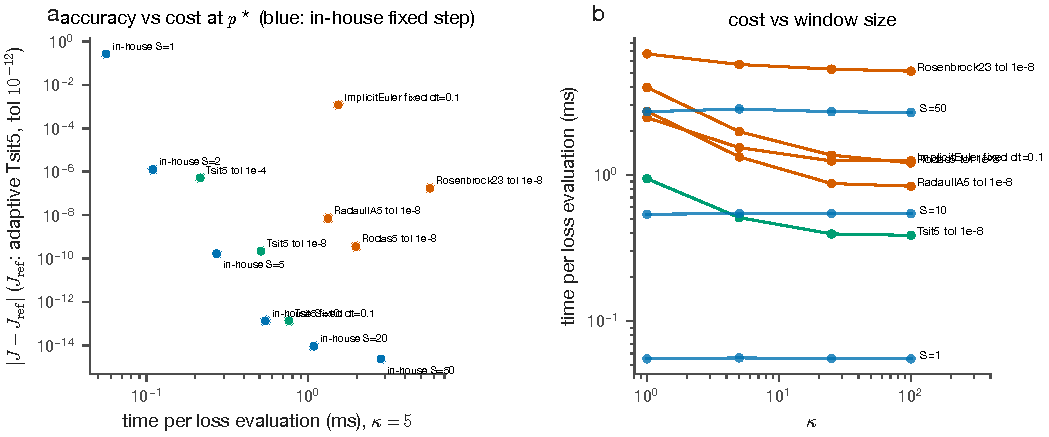
\includegraphics[width=\textwidth]{figures/fig29_solvers_eval.pdf}
\caption{\textbf{Accuracy versus cost of the integrator inside the loss.} (a) $|J-J_{\rm ref}|$ against the time per evaluation at $\kappa=5$, $\pstar$, for the 14 settings of Table~\ref{tab:T3}. The in-house fixed-step Tsit5 at $S=10$ (the default) agrees with the reference to $1.4\times10^{-13}$ at $0.54$\,ms; the adaptive DifferentialEquations Tsit5 at $10^{-8}$ is as accurate at the same cost; implicit solvers (Rosenbrock23, Rodas5, RadauIIA5) cost $3$--$10\times$ more for no gain --- the problem is not stiff; only $S=1$ ($2.7\times10^{-1}$) and fixed-step implicit Euler ($1.2\times10^{-3}$, 9\,\% of $J$) distort the objective. (b) Time per evaluation versus $\kappa$ for a subset. Data: \texttt{solvers\_eval.csv}.}\label{fig:29}\end{figure}

\begin{figure}[H]\centering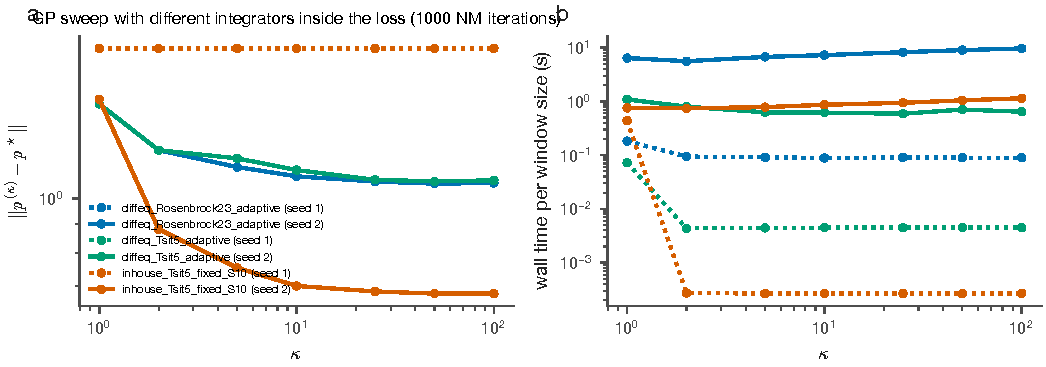
\includegraphics[width=\textwidth]{figures/fig30_solvers_sweep.pdf}
\caption{\textbf{GP sweep with three integrators inside the loss.} In-house Tsit5 ($S=10$), adaptive DifferentialEquations Tsit5 ($10^{-8}$) and Rosenbrock23 ($10^{-8}$), SHORT schedule, 1000 Nelder--Mead iterations, seeds 1 (dotted) and 2 (solid): (a) $\perr$, (b) wall time per stage. Seed 1 is the plateau start and fails identically in all three ($1.84$ at every stage, 0 iterations); seed 2 converges with all three, the two DifferentialEquations arms agreeing exactly at $\kappa\le2$ and diverging afterwards through the chaotic sensitivity of a derivative-free optimiser to $10^{-10}$ differences in the objective (final $0.68$ vs $1.06$--$1.08$ at only 1000 iterations). Rosenbrock23 costs $8\times$ the time. Data: \texttt{solvers\_sweep.csv}.}\label{fig:30}\end{figure}

\section{Part G --- Defects found and fixed}\label{sec:bugs}
Each defect is quantified by executing the frozen pre-fix source (\texttt{deps/prefix/}) against the frozen post-fix source (\texttt{deps/}), never by re-typing; \texttt{analysis/06\_bugs.jl}. Table~\ref{tab:T4} summarises. The fixes are in the live tree in the same commit as this report (every changed line carries the comment \texttt{R002 fix}):

\begin{itemize}[leftmargin=1.4em, itemsep=1pt]
\item \textbf{F1} (R001; \texttt{mod 6}, \texttt{odefun\_new}): the continuation lines beginning with \texttt{+} were separate, discarded statements, so the Jacobian behind the stability/eigenvalue movies was that of the \emph{linear truncation} of the vector field. Fixed by parenthesising the RHS. All movies under \texttt{figs/window\_size\_plots/stability/} are wrong and should be regenerated.
\item \textbf{F2} (R001; \texttt{mod 7} stiff branch of \texttt{forward\_simulation\_loss\_windows}): the same parsing trap dropped the entire $w$-residual. Fixed by parenthesising. (Mod~8 already used a matrix norm and was not affected.)
\item \textbf{F4} (R001; \texttt{mod 7} and \texttt{mod 8} drivers): \texttt{grad\_fs\_loss\_window!} differentiated the single-shooting loss \texttt{fs\_loss}, not \texttt{fs\_loss\_window}. Fixed; this is what makes the BFGS arms of \ref{fig:25} possible.
\item \textbf{F5} (R001; \texttt{plotting\_window\_size.jl}, \texttt{animate\_contourplots!}): stale call signature (missing \texttt{unstable\_param} slot, keyword \texttt{silent} instead of \texttt{silent\_}). Fixed to the mod~6+ signature; \emph{not executed here} (Makie cannot load in the sandbox), so this fix is a reading, not a measurement.
\item \textbf{F6} (R001; \texttt{mod 8} driver): the \texttt{@threads} loop wrote the shared \texttt{x0}, \texttt{results\_inner} and a \texttt{Dict}. Fixed with per-run copies and a lock; not a figure.
\item \textbf{N1 (new)} \texttt{mod 8} driver: the sweep called the pre-refactor \texttt{odefun} (order $1,v,w,\dots$) while the data, \texttt{fhn\_p} and the polish used the library order; the bar-chart labels \texttt{trmstr} encoded the old order and \texttt{plotSolution!} was called with an undefined name \texttt{trm}. The truth vector read in the wrong order is $2.50$ away from itself (\ref{fig:34}a) and its cost at $\kappa=1$ is $0.68$ instead of $0.018$: the committed sweep could not have recovered the model. Fixed (sweep and plots use \texttt{odefun\_generic}; labels generated from \texttt{multiindex\_mapping}).
\item \textbf{N2 (new)} \texttt{mod 8}, \texttt{forward\_simulation\_loss} (explicit branch, used by the final BFGS polish): read the \emph{global} \texttt{data} instead of its \texttt{data\_} argument, so the function ignored the data it was given (\ref{fig:34}b). Fixed. This is the shadowing R001 asked to check when the refactor landed.
\item \textbf{N3 (new, behavioural)} the committed driver had guess propagation \emph{disabled} (\texttt{copyto!(x0, x0\_)} after every stage). Replaced by an explicit \texttt{guess\_mode} switch (\texttt{:propagate} default, \texttt{:best}, \texttt{:reset}).
\item Minor: undefined \texttt{y0} default in \texttt{custom\_integrator}; wrong bound in the window-size warning.
\end{itemize}
R001's bug-presence gates G3, G4, G5 and G7 are retired by this report: R002's gates G5--G9 assert the defects are present in \texttt{deps/prefix/} and absent in \texttt{deps/}.

\begin{table}[H]\centering\small
\caption{Defect quantification (pre-fix vs post-fix frozen sources). From \texttt{bug\_summary.json} and the \texttt{bug\_*.csv} files.}\label{tab:T4}
\begin{tabular}{p{0.36\textwidth} p{0.33\textwidth} p{0.24\textwidth}}
\toprule
finding & measure & value \\
\midrule
F2 (R001): mod 7 stiff branch drops the w-residual & share of J(p*) missing, $\kappa$=1/10/25/100 & 11.5 \% / 9.3 \% / 17.0 \% / 11.2 \% / 11.9 \% \\
F1 (R001): mod 6 odefun\_new = linear truncation & $\partial\dot v/\partial v$ at u=(1.5,0.4): pre-fix vs fixed & 1 vs -1.25 \\
F4 (R001): sweep gradient = single-shooting gradient & cos$\angle$(g$\kappa$, g100) at $\kappa$=1 / 5 & 0.180 / 0.989 \\
NEW: mod 8 driver mixed monomial orders & spurious $\|p-p^\star\|$ between orderings & 2.501 \\
NEW: mod 8 forward\_simulation\_loss ignores data\_ & J identical for 3 datasets pre-fix / differs post-fix & True / True \\
\bottomrule
\end{tabular}

\end{table}

\begin{figure}[H]\centering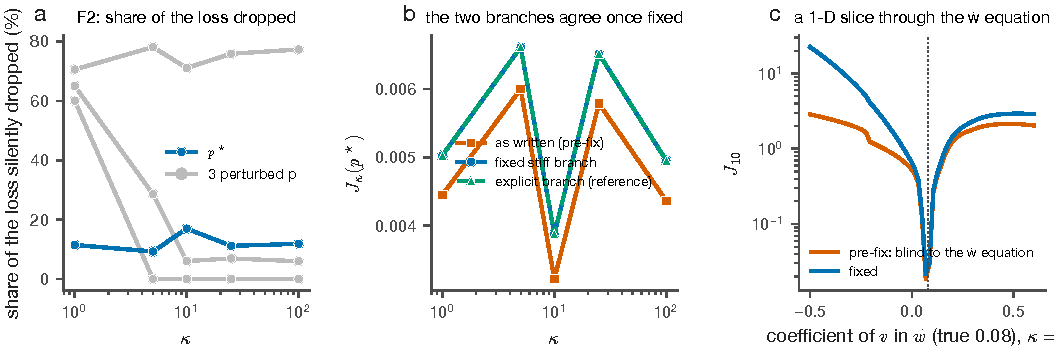
\includegraphics[width=\textwidth]{figures/fig31_bug_F2.pdf}
\caption{\textbf{F2: the mod~7 stiff branch silently discarded the $w$-residual.} (a) Share of the loss missing, $(J_{\rm fixed}-J_{\rm prefix})/J_{\rm fixed}$, at $\pstar$ (blue: $11.5,\,9.3,\,17.0,\,11.2,\,11.9\,\%$ at $\kappa=1,5,10,25,100$, $\gamma=0$) and for three perturbed parameter vectors (grey; up to $78\,\%$ --- away from the optimum the $w$ trajectory is badly wrong and the dropped term dominates; rows at $0$ are blow-ups, where both versions return $10^3$). (b) The three implementations at $\pstar$: pre-fix stiff branch, fixed stiff branch and the explicit in-house branch agree to $3\times10^{-10}$ once fixed. (c) A 1-D slice through the $v$ coefficient of the $\dot w$ equation at $\kappa=10$: the fixed objective varies by a factor $10^3$ across the slice, the pre-fix one barely moves --- the stiff branch was blind to the $\dot w$ equation, so every contour/surface movie made with \texttt{stiff\_solver\_=true} shows the wrong landscape. Data: \texttt{bug\_F2\_w\_residual.csv}, \texttt{bug\_F2\_slice.csv}.}\label{fig:31}\end{figure}

\begin{figure}[H]\centering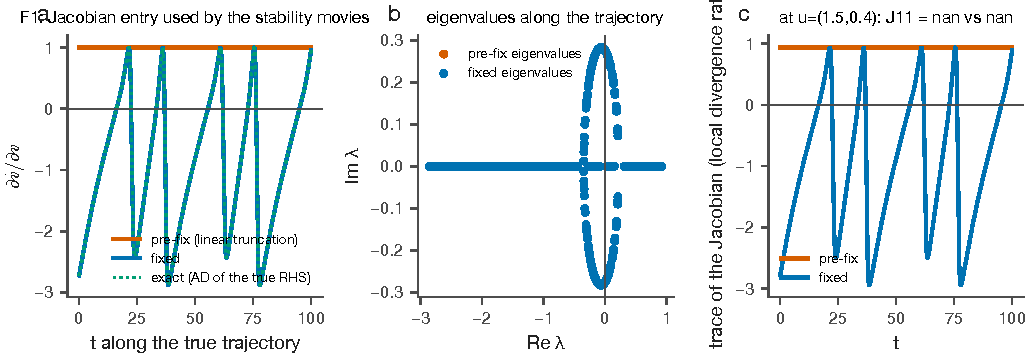
\includegraphics[width=\textwidth]{figures/fig32_bug_F1.pdf}
\caption{\textbf{F1: the stability movies used a linear truncation of the vector field.} Along the true FHN trajectory (401 points): (a) $\partial\dot v/\partial v$ from the pre-fix \texttt{odefun\_new} (vermilion, constant $+1$), the fixed one (blue) and the exact Jacobian of the true RHS (green dotted, identical to fixed to $0.0$); at $u=(1.5,0.4)$ the entry is $+1.0$ instead of $-1.25$ --- the wrong sign. (b) Jacobian eigenvalues along the orbit, pre-fix (a fixed pair) versus fixed (moving with the state, crossing into the stable half-plane on the slow branches). (c) The trace (local divergence rate), constant and positive pre-fix, mostly negative after the fix. Data: \texttt{bug\_F1\_jacobian.csv}, \texttt{bug\_F1\_meta.json}.}\label{fig:32}\end{figure}

\begin{figure}[H]\centering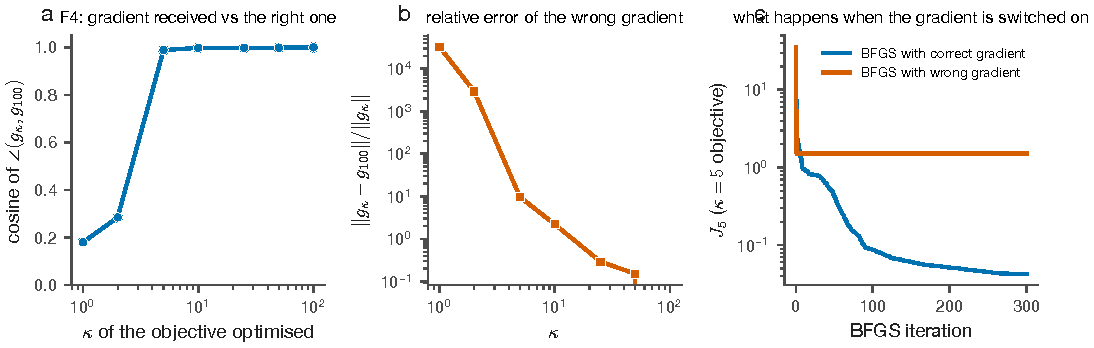
\includegraphics[width=\textwidth]{figures/fig33_bug_F4.pdf}
\caption{\textbf{F4: the sweep's gradient was the gradient of the wrong function.} At $z=[y_0;\,\pstar+0.05\,\xi]$: (a) cosine between the gradient of the $\kappa$-windowed objective and the single-shooting gradient the pre-fix code returned --- $0.18$ at $\kappa=1$ ($80^\circ$), $0.99$ at $\kappa=5$, $1$ at $\kappa=100$; (b) the relative error of the wrong gradient, $3\times10^4$ at $\kappa=1$ (the single-shooting gradient is huge because that trajectory has diverged). (c) 300 BFGS iterations on the $\kappa=5$ objective from the same start with the correct gradient ($J_5$: $35.8\to0.043$) and with the wrong one (stalls at $1.51$ from iteration 19, 23\,708 line-search evaluations). The defect was harmless only because the sweep used Nelder--Mead, which ignores the gradient. Note: this start ($\perr=0.23$) has a large cost because the $0.05$ perturbation hits the cubic term; the correct-gradient run lowers $J_5$ but ends at $\perr=3.96$ (a different, wrong minimum) --- the panel demonstrates the gradient, not recovery. Data: \texttt{bug\_F4\_gradient.csv}, \texttt{bug\_F4\_bfgs.csv}.}\label{fig:33}\end{figure}

\begin{figure}[H]\centering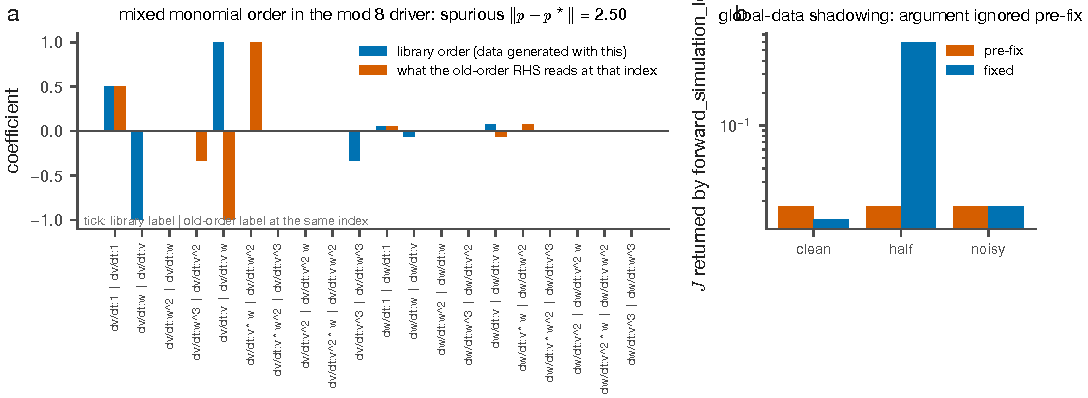
\includegraphics[width=\textwidth]{figures/fig34_bug_ordering_shadowing.pdf}
\caption{\textbf{New defects in the committed mod~8 driver.} (a) N1, mixed monomial order: the true coefficients in the library order the data were generated with (blue) and what the old-order RHS used by the sweep reads at the same index (vermilion); tick labels give both names. The two readings of the same vector are $2.50$ apart (larger than $\lVert\pstar\rVert=1.54$), and the true vector evaluated through the old-order RHS costs $0.68$ ($\kappa=1$), $2.06$ ($\kappa=5$), $7.83$ ($\kappa=100$) instead of $0.018$--$0.021$. (b) N2, global-data shadowing: \texttt{forward\_simulation\_loss} called with three different data matrices (noisy, clean, states halved) returns the same $0.0176$ pre-fix and $0.0176$ / $0.0133$ / $0.592$ after the fix. Data: \texttt{bug\_ordering.csv}, \texttt{bug\_ordering\_meta.json}, \texttt{bug\_shadowing.csv}.}\label{fig:34}\end{figure}

\section{Part H --- Other systems and closing the loop with the theory}\label{sec:other}
The core is dimension- and degree-agnostic; two further systems test it (Table~\ref{tab:T5}). Lotka--Volterra: $\dot x=x-0.5xy$, $\dot y=-0.8y+0.3xy$, quadratic library (6 monomials, 12 coefficients), $N=101$, $\Delta t=0.25$, 5\,\% noise, Nelder--Mead. Lorenz: $\sigma=10,\rho=28,\beta=8/3$, quadratic library (10 monomials, 30 coefficients), $N=101$, $\Delta t=0.02$ ($t\in[2,4]$ of a trajectory from $(-8,7,27)$), 2\,\% noise, start scale $0.5$; BFGS (2500-iteration cap) and Nelder--Mead (4000). Same SHORT schedule and $\gamma=0.05$.

\begin{table}[H]\centering\small
\caption{Other systems at $\kappa=100$: seed medians of $\perr$ and score, and the fraction of seeds on the plateau. From \texttt{other\_sweeps.csv}.}\label{tab:T5}
\input{tables/T5_other_systems}
\end{table}

\begin{figure}[H]\centering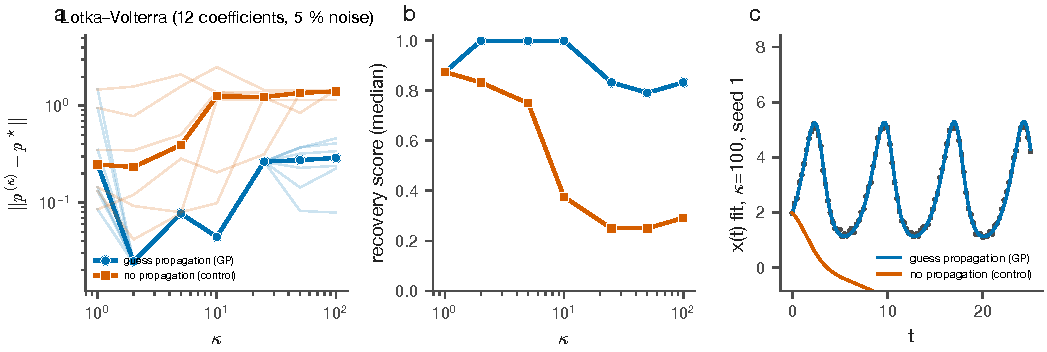
\includegraphics[width=\textwidth]{figures/fig35_lotka_volterra.pdf}
\caption{\textbf{Lotka--Volterra.} (a) $\perr$ along the sweep (thin: 6 seeds, thick: median), (b) score, (c) the $x(t)$ fit at $\kappa=100$ for seed 1. GP ends at $0.29$ (score $0.83$; one seed reaches $0.025$ with score $1.0$ at $\kappa=2$--$10$, i.e.\ exact recovery), the control at $1.41$ with 5 of 6 seeds on the plateau; GP is better in every seed. Data: \texttt{other\_sweeps.csv}, \texttt{other\_fits.csv} (\texttt{system=lv}).}\label{fig:35}\end{figure}

\begin{figure}[H]\centering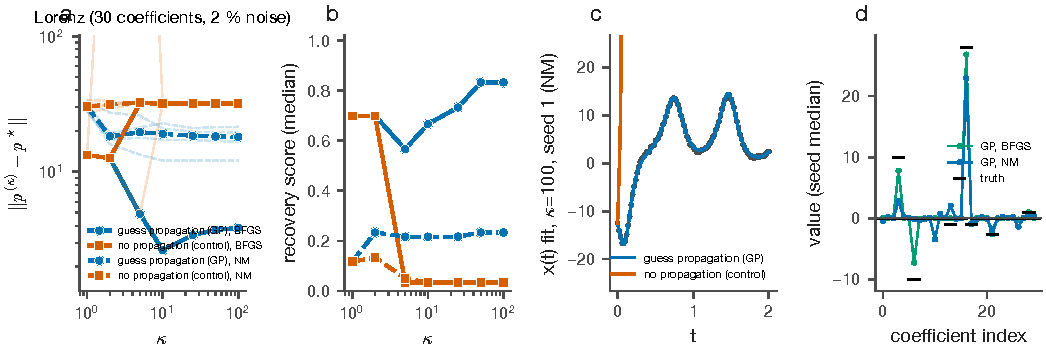
\includegraphics[width=\textwidth]{figures/fig36_lorenz.pdf}
\caption{\textbf{Lorenz (chaotic, 30 coefficients).} (a) $\perr$ along the sweep for BFGS (solid) and Nelder--Mead (dashed), GP (blue) and control (vermilion), 4 seeds; (b) score; (c) the $x(t)$ fit at $\kappa=100$, seed 1; (d) the seed-median GP coefficients versus truth. GP+BFGS recovers Lorenz ($\perr=3.9$ on coefficients of size up to 28, score $0.83$, no blow-up); GP+Nelder--Mead never converges within 4000 iterations in 33 dimensions ($18.1$, score $0.23$) --- a derivative-free sweep does not scale; the control blows up in 4 of 4 seeds from $\kappa=5$ on with either optimiser. Data: \texttt{other\_sweeps.csv}, \texttt{other\_minimizers.csv}, \texttt{other\_fits.csv} (\texttt{system=lorenz}).}\label{fig:36}\end{figure}

\begin{figure}[H]\centering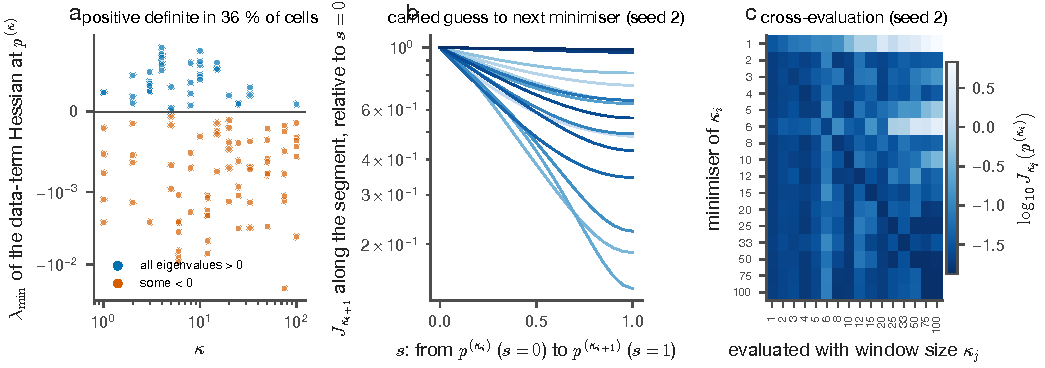
\includegraphics[width=\textwidth]{figures/fig37_post_hessian_path.pdf}
\caption{\textbf{The theory's premises checked where they are assumed.} (a) Smallest eigenvalue of the data-term Hessian at the GP minimiser $p^{(\kappa)}$ returned by Nelder--Mead at every stage, 7 seeds (the plateau seed excluded; symlog scale; blue = all 20 eigenvalues positive, vermilion = at least one negative). Where the manuscript assumes local strong convexity --- at the minimiser, not at $\pstar$ --- the returned point is positive definite in only 36\,\% of the (seed, $\kappa$) cells, with on average $0.8$ of 20 eigenvalues slightly negative elsewhere ($|\lambda_{\min}|\lesssim10^{-3}$ against $\lambda_{\max}$ of $10$--$10^6$): Nelder--Mead stops short of a true stationary point in 22 dimensions (cf.\ \ref{fig:27}a), so the premise is \emph{not} verified at the returned iterates; the BFGS iterates of \ref{fig:25} would be the right place to test it. (b) The cost of the \emph{next} stage along the straight segment from $p^{(\kappa_i)}$ to $p^{(\kappa_{i+1})}$ (seed 2), relative to its value at the carried guess: it decreases monotonically along every segment, i.e.\ the carried guess lies inside the basin of the next minimiser --- the mechanism the node-removal theorem describes. (c) Cross-evaluation (seed 2): the minimiser of $\kappa_i$ evaluated at every other $\kappa_j$ (log colour); the near-diagonal structure shows that a minimiser is good only for nearby window sizes, which is why the schedule must be gradual (\ref{fig:21}). Data: \texttt{post\_hessian\_at\_minimizers.csv}, \texttt{post\_path\_between\_minimizers.csv}, \texttt{post\_cross\_evaluation.csv}.}\label{fig:37}\end{figure}

\section{Part I --- Extended landscape animations: plane selection, resolution, and 3-D}\label{sec:anim2}
The landscape animation of Part~C (\texttt{anim\_fhn\_landscape.mp4}) shows one FHN coefficient plane at
$61\times61$. This part extends it to five FHN planes and one Lotka--Volterra plane at $201\times201$,
adds a rotating 3-D version of four of them, and --- because ``pick an interesting plane'' is exactly
the kind of choice that invites cherry-picking --- states the rule by which the planes were chosen and
shows the evidence for every candidate, selected or not.

\subsection{Definitions used in this part}\label{sec:anim2defs}
Everything below is defined here; nothing is inherited implicitly.
\begin{itemize}[leftmargin=1.4em, itemsep=1pt]
\item \textbf{Coefficient plane $\Pi(i,j)$.} The two-dimensional slice of parameter space on which the
coefficients $p_i$ and $p_j$ sweep a rectangle centred on their true values $p^\star_i,p^\star_j$ while
\emph{all other coefficients are held at the truth} ($18$ of them for FHN, $10$ for Lotka--Volterra) and
the initial state is the first datum. A plane is named by its two library monomials and the state
equation each sits in, e.g.\ $\Pi(v\ \text{in}\ \dot v,\ v^3\ \text{in}\ \dot v)$. Parameter indices follow the
library ordering of \S\ref{sec:defs}: $1,w,w^2,w^3,v,vw,vw^2,v^2,v^2w,v^3$ for the $\dot v$ block
($p_1$--$p_{10}$), then the same ten monomials for the $\dot w$ block ($p_{11}$--$p_{20}$).
\item \textbf{Cost $J_\kappa$.} Exactly the multiple-shooting cost of \S\ref{sec:defs} with $\gamma=0.05$,
$S=10$, $\delta t=0.1$ and window size $\kappa$; it returns the flat value $10^3$ on finite-time blow-up.
\item \textbf{Plateau fraction $\varphi_\kappa$.} The fraction of the plane's grid cells with
$J_\kappa\ge10^3$: the share of the plane on which the model blows up before the record ends.
\item \textbf{Basin fraction $\beta_\kappa$.} The fraction of grid cells with
$J_\kappa<2\min_\Pi J_\kappa$ --- the visible area of the valley around the best point of the plane.
It is an \emph{area}, not a width: $\beta$ falling by $10\times$ means the valley floor is $10\times$
smaller in area, roughly $3\times$ narrower in each direction.
\item \textbf{Dynamic range $D_\kappa$.} $\log_{10}\!\big(\max J_\kappa/\min J_\kappa\big)$ over the
cells that do \emph{not} blow up, in decades. Small $D$ means a nearly flat plane: the cost barely
distinguishes the truth from anything else on it.
\item \textbf{Rank decorrelation $1-\rho_{1,100}$.} $\rho_{1,100}$ is the Spearman (rank) correlation
between $\log J_1$ and $\log J_{100}$ over the cells that are finite at \emph{both} $\kappa=1$ and
$\kappa=100$. It is $0$ when the two landscapes order the plane identically and $2$ when they order it
exactly oppositely; a value above $1$ therefore means the ranking has \emph{inverted} --- points that
$\kappa=1$ prefers, $\kappa=100$ rejects.
\item \textbf{Censoring floor.} On the $61\times61$ screening grid the smallest measurable $\beta$ is
one cell, $1/61^2=0.027\,\%$. Eight of the sixteen candidate planes sit at exactly that value at
$\kappa=100$, so the implied basin ratios $\beta_1/\beta_{100}$ of those rows in Table~\ref{tab:T6} are
\emph{lower bounds}, not measurements. Table~\ref{tab:T7} re-measures the five animated planes on the
$201\times201$ production grid, where the floor is $1/201^2=0.0025\,\%$ and only one cell of the whole
table --- the basin of $\Pi(w\ \text{in}\ \dot v,\ v\ \text{in}\ \dot w)$ at $\kappa=100$ --- still
sits on it.
\end{itemize}

\subsection{How the planes were chosen}
All $16$ candidate planes of Table~\ref{tab:T6} were scanned at $61\times61$ over the full $\kappa$
ladder ($\kappa\in\{1,2,3,4,5,6,8,10,12,15,20,25,33,50,75,100\}$) by
\pathtt{analysis/12_landscape_planes.jl}; the table is the complete screen, with no candidate omitted.
Five planes were animated, each the extreme case of one \emph{distinct} mechanism by which the
landscape changes with $\kappa$:
\begin{itemize}[leftmargin=1.4em, itemsep=1pt]
\item $\Pi(v\ \text{in}\ \dot v,\ v^3\ \text{in}\ \dot v)$ --- the plane already animated in Part~C, kept for
continuity and re-rendered at $201\times201$. It has the largest rank decorrelation of all sixteen
($1-\rho=1.22$): the ordering of the plane inverts between $\kappa=1$ and $\kappa=100$.
\item $\Pi(v\ \text{in}\ \dot w,\ w\ \text{in}\ \dot w)$ --- the slow block. Largest basin collapse of all
sixteen: on the $201\times201$ production grid $\beta$ falls from $8.94\,\%$ of the plane at $\kappa=1$ to $0.0050\,\%$ (two cells) at $\kappa=100$ --- more than $1800\times$, the largest collapse in the set (Table~\ref{tab:T7}); it also has the largest gain in dynamic range ($1.53\to4.74$ decades).
\textbf{Read this:} at $\kappa=1$ this plane is nearly flat --- one-interval shooting barely constrains
the slow subsystem at all --- and by $\kappa=100$ it is a narrow canyon with a blow-up wall along one
side. This is the most drastic transformation in the screen.
\item $\Pi(v^2\ \text{in}\ \dot v,\ v^2\ \text{in}\ \dot w)$ --- two coefficients that are \emph{zero} in the
truth. Largest growth of the blow-up plateau in the screen, $\varphi$ from $0\,\%$ to $57\,\%$ of the
plane, with $D$ from $2.17$ to $4.75$ decades. This is the plane on which the spurious quadratic terms
that sparse selection must reject are penalised, and it shows that long windows do the rejecting by
making those terms \emph{blow up} rather than by making them merely expensive.
\item $\Pi(w\ \text{in}\ \dot v,\ v\ \text{in}\ \dot w)$ --- the FHN feedback pair, and the control case:
it barely blows up at all. On the $201\times201$ grid $\varphi$ is exactly zero for every $\kappa\le33$, is a single cell ($0.0025\,\%$) at $\kappa=50$, and reaches only $0.16\,\%$ and $0.27\,\%$ of the plane at $\kappa=75$ and $\kappa=100$, against $28$--$60\,\%$
for the other four planes; yet its dynamic range still grows from $1.93$ to $4.54$ decades, the largest
gain among the planes the screen records with no plateau. Sharpening and plateau growth are separate
mechanisms, and this plane isolates the first.
\item $\Pi(v^3\ \text{in}\ \dot v,\ v^3\ \text{in}\ \dot w)$ --- twin cubic terms. Already rugged at
$\kappa=1$ ($\varphi=32\,\%$, $D=4.71$) and the most blown-up plane at $\kappa=100$ ($\varphi=60\,\%$):
ruggedness on top of ruggedness, the least favourable case for an optimiser.
\end{itemize}
\readthis{The selection rule is ``extreme on a named mechanism'', not ``largest composite score'', and
several unselected planes beat selected ones on individual columns: $\Pi(1\ \text{in}\ \dot v,\ 1\ \text{in}\
\dot w)$ and $\Pi(w\ \text{in}\ \dot v,\ w^3\ \text{in}\ \dot v)$ have larger (censored) basin ratios than
$\Pi(w\ \text{in}\ \dot v,\ v\ \text{in}\ \dot w)$, and $\Pi(v^3\ \text{in}\ \dot v,\ vw\ \text{in}\ \dot v)$ has a
larger rank decorrelation than three of the five selected. Table~\ref{tab:T6} is printed in full so that
the choice can be second-guessed.}

\begin{table}[H]\centering\small
\caption{\textbf{The complete landscape-plane screen} (FHN, $61\times61$, all 16 candidates, none
omitted). Columns as defined in \S\ref{sec:anim2defs}: rank decorrelation $1-\rho_{1,100}$, basin
fraction $\beta_\kappa$ and plateau fraction $\varphi_\kappa$ at the two ends of the ladder, and the
dynamic range $D_\kappa$ in decades. A basin of $0.027\,\%$ is exactly one grid cell --- the censoring
floor of this grid --- so the implied shrink factors of those rows are lower bounds;
Table~\ref{tab:T7} re-measures the animated planes without censoring. ``animated'' marks the five planes
carried to $201\times201$. Data: \texttt{landscape\_plane\_screen\_summary.csv}, script
\texttt{analysis/12\_landscape\_planes.jl}.}
\label{tab:T6}
\input{tables/T6_landscape_plane_screen}
\end{table}

\subsection{Resolution}
The production grids are $201\times201$ at every one of the $16$ window sizes: $10.9\times$ the samples
of the $61\times61$ grid behind the Part~C animation and $1.6\times$ the $161\times161$ Lotka--Volterra
grids, i.e.\ $646\,416$ cost evaluations per plane. Frames are rendered at $2560\times1440$ (1440p)
rather than the previous $825\times616$ --- $7.2\times$ the pixels. The grids are stored gzipped
(\texttt{.csv.gz}, read directly by pandas): a plain-text $201\times201\times16$ grid is about $18$\,MB
and compresses to $3$--$4$\,MB. Table~\ref{tab:T7} reports the geometry of the five animated planes
measured on \emph{these} grids; these, not the screening numbers, are what the videos show.

\begin{table}[H]\centering\small
\caption{\textbf{The animated planes at production resolution} ($201\times201$; $\beta_\kappa$ and
$\varphi_\kappa$ as in \S\ref{sec:anim2defs}). One value is censored, and only one: the basin of
$\Pi(w\ \text{in}\ \dot v,\ v\ \text{in}\ \dot w)$ at $\kappa=100$ is a single cell,
$1/201^2=0.0025\,\%$, so the shrink factor printed for that row is a lower bound; every other basin in
the table is two cells or more and is measured. Column ``3-D'' marks the four planes that also have a
rotating 3-D animation; ``key'' is the file-name stem --- the 2-D video of a row is
\texttt{anim\_fhn\_landscape\_<key>\_hires.mp4} (\texttt{anim\_lv\_landscape\_x2\_xy\_hires.mp4} for the
Lotka--Volterra row) and its 3-D video, where it exists, is \texttt{anim3d\_fhn\_landscape\_<key>.mp4}
(\texttt{anim3d\_lv\_landscape\_x2\_xy.mp4}). $J^{\min}_\kappa$ is the
smallest cost anywhere on the plane at that $\kappa$; it is not in general attained at $p^\star$,
because the data carry $5\,\%$ noise. Data: \texttt{landscape\_hires\_geometry.csv}, written by
\texttt{figures/make\_landscape\_animations.py} from the same grids the frames are drawn from.}
\label{tab:T7}
\input{tables/T7_animated_planes}
\end{table}

\subsection{The 3-D animations}
Four planes are additionally rendered as a rotating 3-D surface $z=\log_{10}J_\kappa$: the two most
drastic FHN planes ($\Pi(v\ \text{in}\ \dot w,\ w\ \text{in}\ \dot w)$ and
$\Pi(v^2\ \text{in}\ \dot v,\ v^2\ \text{in}\ \dot w)$), the Part~C plane
$\Pi(v\ \text{in}\ \dot v,\ v^3\ \text{in}\ \dot v)$ for continuity, and the Lotka--Volterra $(x^2,xy)$ plane
of $\dot x$. Each animation holds one $\kappa$ for $16$ frames (the first and last for $32$) while the
camera azimuth advances, completing one full turn over the $288$ frames; the guess-propagation and
control paths walk over the surface with their shadow on the floor, and the floor carries a filled
contour projection of the same surface.
\readthis{\textbf{Display convention.} The 3-D surface is $\log_{10}J_\kappa$ \emph{clipped} at the
$99.5$th percentile of the finite costs on that plane, and cells on the blow-up plateau are drawn as a
flat grey mesa at that ceiling. Without the clip the blow-up value $10^3$ --- three decades above the
bulk of the plane --- owns most of the vertical axis and flattens the valley the picture is about. The
clip changes the \emph{height and colour of this one drawn surface} only: no cost value is altered
anywhere else in this report, the 2-D animations are unclipped, and the plateau is still identified by
colour and named in every frame's subtitle.}

\subsection{The same plane without guess propagation}
\texttt{anim3d\_fhn\_landscape\_wv\_ww\_control.mp4} is the slow-block 3-D animation with the
guess-propagation path deleted: the only trajectory left is the \emph{control} arm, i.e.\ the
minimiser $p^{(\kappa)}$ the optimiser returns at each window size when every stage restarts from
the same seed vector rather than from the previous stage's answer. It is the picture of what the
window-size ladder does on its own, before guess propagation is introduced, and it is the natural
companion to the two-arm version: the surface tightens into a canyon exactly as before, but the
returned minimiser never settles into it --- the projected iterate jumps across the plane from one
$\kappa$ to the next, and the gutter panel shows $\lVert p^{(\kappa)}-p^\star\rVert$ oscillating
between $1.43$ and $1.95$ with no trend along the ladder, on both sides of the shared starting
guess ($1.52$; below it in $6$ of the $16$ stages) and ending at $1.55$ --- no better than the
$1.44$ it already had at $\kappa=1$. Lengthening the windows alone buys nothing: it is the
\emph{carried guess} that converts the tightening landscape into a better parameter estimate.
\readthis{The control minimiser and the minimum \emph{of the drawn plane} are different objects and
must not be read as the same marker. $\arg\min_\Pi J_\kappa$ is the best point of a slice whose
other $18$ coefficients are pinned at the truth; on this plane it sits on the truth star at
$(0.080,-0.060)$ for every $\kappa$ in the ladder, to within one grid cell. The control minimiser is
a full $20$-dimensional optimiser output projected onto the plane, and over the ladder it sits
between $0.08$ and $0.47$ away from the truth. A renderer mode for the former exists
(\texttt{make\_landscape\_animations.py 3d-min}) but is not shipped as a video, because a marker
pinned to the truth star carries no motion worth animating.}

\subsection{What the animations do and do not show}
\begin{itemize}[leftmargin=1.4em, itemsep=1pt]
\item \textbf{The surface and the path live in different spaces.} The landscape holds the other $18$
(FHN) or $10$ (LV) coefficients at the truth, whereas each plotted path point is the projection of a
full $20$- or $12$-dimensional minimiser whose other coefficients are \emph{not} at the truth. A path
point can therefore sit visibly off the valley floor of the drawn surface without either being wrong.
This caveat applies equally to the Part~C animation.
\item \textbf{Ladder mismatch.} The FHN paths (seed 2) visit all $16$ window sizes of the FULL schedule,
so the path advances in every frame. The Lotka--Volterra sweep was run on the SHORT schedule, so its
path advances only at the window sizes SHORT contains and is stationary in the intervening frames; the
surface still morphs at every $\kappa$.
\item \textbf{At $\kappa=1$ the two arms coincide} by construction --- guess propagation has nothing to
propagate yet --- so the blue marker is hidden under the vermilion one in the first frame.
\item \textbf{These are slices, not the optimisation landscape.} Nothing here shows the $22$-dimensional
geometry the optimiser actually traverses; $\beta_\kappa$ and $\varphi_\kappa$ are properties of a
two-dimensional cut, and the basin collapse they report is not a statement about the volume of the full
basin.
\end{itemize}

\section{Gates}\label{sec:gates}
\pathtt{analysis/verify_R002.py} reads only this folder's own result files and writes \pathtt{analysis/results/gates_summary.json}. \textbf{Status at the final build: 20 of 20 gates pass
.} Gates G5--G9 are bug-presence/absence gates (pre-fix present, post-fix absent); they are expected to keep passing as long as \texttt{deps/prefix/} is the \texttt{44abf4a} snapshot. All other gates are ordinary correctness or completeness gates.
\begin{center}\small
\begin{tabular}{lp{0.78\textwidth}}
\toprule
gate & asserts \\
\midrule
G1 & all 12 frozen files hash to \texttt{deps/MANIFEST.md} \\
G2 & \texttt{ms\_loss} = frozen mod~8 loss, relative difference $<10^{-10}$ (42 evaluations) \\
G3 & dataset = frozen mod~8 data block, $<10^{-12}$ \\
G4 & \texttt{make\_rhs} = \texttt{odefun\_poly!} and = old-order \texttt{odefun} under the permutation, $<10^{-12}$ \\
G5 & F1 present pre-fix ($\partial\dot v/\partial v=+1.0$), absent post-fix ($-1.25$ = exact, max deviation 0) \\
G6 & F2 present pre-fix (5--25\,\% of $J(\pstar)$ missing at every $\kappa$), fixed stiff = explicit to $10^{-8}$ \\
G7 & F4 present pre-fix: cosine $<0.5$ at $\kappa=1$ and $>0.999$ at $\kappa=100$ \\
G8 & N1 present pre-fix: spurious $\perr>1$; old-order cost of $\pstar$ $>10\times$ the correct one \\
G9 & N2 present pre-fix (identical $J$ for 3 datasets), absent post-fix \\
G10 & main sweep complete: 3 arms $\times$ 8 seeds $\times$ 16 stages = 384 rows \\
G11 & GP tied with control at $\kappa=1$ in every seed and strictly better in every non-plateau seed at every $\kappa\ge2$ \\
G12 & paired GP $-$ control CI at $\kappa=100$ excludes 0 \\
G13 & every control row on the plateau returns exactly the seed vector \\
G14 & in-house $S=10$ loss within $10^{-8}$ of the adaptive reference at $\kappa\in\{1,5,25,100\}$ \\
G15 & other systems: GP better than control in every seed (LV, Lorenz BFGS, Lorenz NM) \\
G16 & every planned sweep job realised \\
G17 & every figure referenced by \texttt{report.tex} exists; results ledger written \\
G18 & Table~\ref{tab:T1}'s medians reproduce from \texttt{sweeps.csv} \\
G19 & the extended landscape animation set is complete: 16 candidate planes screened, 5 animated, 6 two-dimensional and 4 three-dimensional MP4s present and non-trivial \\
G20 & the basin and plateau fractions of Table~\ref{tab:T7} (and of every animation frame) recompute from the shipped $201\times201$ grids, all 96 (plane, $\kappa$) cells \\
\bottomrule
\end{tabular}
\end{center}

\section{Limitations and honest notes}
\begin{itemize}[leftmargin=1.4em, itemsep=1pt]
\item \textbf{Seeds.} 8 optimiser seeds (6 for noise/sparsity, 4 for iterations/sub-steps/Lorenz, 10 starts per radius for the basin experiment) is enough for paired CIs that exclude zero, not for tail statistics; one seed in eight starts on the plateau and is kept in every median.
\item \textbf{Nelder--Mead budget.} At 2500 iterations the sweep is converged for FHN (\ref{fig:27}a) but not for Lorenz (\ref{fig:36}); the BFGS arms are the recommendation, and their wall times are machine-dependent.
\item \textbf{The Lipschitz bounds are loose} by orders of magnitude on this attracting system (\ref{fig:08}--\ref{fig:10}); the figures support the theory's \emph{ordering} of single vs multiple shooting, not the size of the constants.
\item \textbf{Not gated:} F5 (Makie) and F6 (a race) are readings; the concept figures 3 and 7 are schematics and say so.
\item \textbf{Timing columns} are wall-clock on a shared 16-core machine with up to 16 concurrent processes and are only comparative.
\item \textbf{Planned vs realised.} 522 planned sweep jobs; the batch was re-sharded twice (resume logic in \texttt{04\_sweeps.jl}) after two shards stalled on slow L-BFGS jobs; duplicates from deterministic re-runs are removed at merge time (identical results, different wall time). The first-batch sparsity jobs (arm name without $\gamma$) were superseded by $\gamma$-named arms and are dropped at merge.
\end{itemize}

\section*{Reproduction}
\addcontentsline{toc}{section}{Reproduction}
See \texttt{REPRODUCE.md} for the pinned environment and the ordered commands (Julia stages 00--12, then the Python inventory, tables, figures, animations, gates, number manifest, and \texttt{pdflatex} twice). \texttt{report.md} is a full-content Markdown rendition of this document generated from the same sources.
\end{document}
